\documentclass[12pt,a4paper]{article}
\usepackage{pgfgantt}
\usepackage{rotating}
\usepackage{fullpage}
\usepackage{float}
\usepackage{texments}
\usepackage[T1]{fontenc}
\usepackage{listings}
\usepackage{verbatim}
\usepackage[utf8]{inputenc}
\usepackage{amsfonts}
\usepackage{amssymb}
\usepackage{listings}
\usepackage[french,english]{babel}
\usepackage[cyr]{aeguill}
\usepackage[hyphens,spaces,obeyspaces]{url}
\usepackage[colorlinks,allcolors=blue]{hyperref}
\usepackage[super]{natbib}
\usepackage{graphicx}
\usepackage{lscape}
\usepackage{xcolor}
\usepackage{sectsty}
\usepackage{cleveref}
\chapterfont{\color{blue!50!blac}}  
\sectionfont{\color{blue!50!black}}  
\subsectionfont{\color{red!50!black}}  
\subsubsectionfont{\color{green!50!black}}  
\bibliographystyle{plainnat}  

\def\dollar{\$}

\setlength{\parindent}{2em}
\setlength{\parskip}{1em}
\newcommand{\quotes}[1]{``#1''}
\def\dollar{\$}

\setlength{\parindent}{2em}
\setlength{\parskip}{1em}

\usepackage{listings}
\usepackage{color}
\definecolor{lightgray}{rgb}{.9,.9,.9}
\definecolor{darkgray}{rgb}{.4,.4,.4}
\definecolor{purple}{rgb}{0.65, 0.12, 0.82}



\usepackage{xcolor}

\definecolor{Zgris}{rgb}{0.87,0.85,0.85}

\newsavebox{\BBbox}
\newenvironment{DDbox}[1]{
\begin{lrbox}{\BBbox}\begin{minipage}{\linewidth}}
{\end{minipage}\end{lrbox}\noindent\colorbox{Zgris}{\usebox{\BBbox}} \\
[.5cm]}

\lstdefinelanguage{JavaScript}{
  keywords={typeof, new, true, false, catch, function, return, null, catch, switch, var, if, in, while, do, else, case, break},
  keywordstyle=\color{blue}\bfseries,
  ndkeywords={class, export, boolean, throw, implements, import, this},
  ndkeywordstyle=\color{darkgray}\bfseries,
  identifierstyle=\color{black},
  sensitive=false,
  comment=[l]{//},
  morecomment=[s]{/*}{*/},
  commentstyle=\color{purple}\ttfamily,
  stringstyle=\color{red}\ttfamily,
  morestring=[b]',
  morestring=[b]"
}

\lstset{
   language=JavaScript,
   backgroundcolor=\color{lightgray},
   extendedchars=true,
   basicstyle=\footnotesize\ttfamily,
   showstringspaces=false,
   showspaces=false,
   numbers=left,
   numberstyle=\footnotesize,
   numbersep=9pt,
   tabsize=2,
   breaklines=true,
   showtabs=false,
   captionpos=b
}
\newcommand{\HRule}{\rule{\linewidth}{0.5mm}}
%python
% Default fixed font does not support bold face
\DeclareFixedFont{\ttb}{T1}{txtt}{bx}{n}{12} % for bold
\DeclareFixedFont{\ttm}{T1}{txtt}{m}{n}{12}  % for normal

% Custom colors
\usepackage{color}
\definecolor{deepblue}{rgb}{0,0,0.5}
\definecolor{deepred}{rgb}{0.6,0,0}
\definecolor{deepgreen}{rgb}{0,0.5,0}

\usepackage{listings}

% Python style for highlighting
\newcommand\pythonstyle{\lstset{
language=Python,
basicstyle=\ttm,
otherkeywords={self},             % Add keywords here
keywordstyle=\ttb\color{deepblue},
emph={MyClass,__init__},          % Custom highlighting
emphstyle=\ttb\color{deepred},    % Custom highlighting style
stringstyle=\color{deepgreen},
frame=tb,                         % Any extra options here
showstringspaces=false            % 
}}


% Python environment
\lstnewenvironment{python}[1][]
{
\pythonstyle
\lstset{#1}
}
{}

% Python for external files
\newcommand\pythonexternal[2][]{{
\pythonstyle
\lstinputlisting[#1]{#2}}}

% Python for inline
\newcommand\pythoninline[1]{{\pythonstyle\lstinline!#1!}}

\begin{document}
\begin{titlepage}
\begin{center}

{\scshape\LARGE Université de Bordeaux \par}
{\scshape\Large Master 1 Informatique \par}

\vspace{3cm}
\HRule \\[0.4cm]
{\Huge\bfseries Projet de programmation \par}%%%%
\HRule \\
{\Large\itshape Réalité augmentée \par}
\vspace{3cm}

\begin{minipage}{.46\linewidth}
	\begin{flushleft} \large
    	{\bfseries Réalisé par} \par
    	\begin{itemize}
          \item Aghiles \textsc{CHAOUCHI}
          \item Nadhir \textsc{HOUARI} 
          \item Anas \textsc{BELMEKKI} 
          \item El Mehdi \textsc{KHACHIR}
    	\end{itemize}
	\end{flushleft}
\end{minipage}
\begin{minipage}{.46\linewidth}
	\begin{flushleft} \large
    	{\bfseries Chargé de TD} \par
		\begin{itemize}
      		\item Pascal \textsc{DESBARATS}
    	\end{itemize}
		{\bfseries Clients} \par
         \begin{itemize}
         	\item Adrien \textsc{BOUSSICAULT}
      		\item Pierre \textsc{LACROIX}
    	\end{itemize}
   \end{flushleft}
\end{minipage}
\vfill
\vfill
{\large 08 janvier 2017\par}
\end{center}
\end{titlepage}
\tableofcontents
\newpage
%Introduction
\section{Introduction}

Dans la vie courante, il y a des taches qui peuvent nous sembler simples, en  réalité elles sont compliquées pour certaines personnes, alors la domotique nous a permis de les automatiser et de les simplifier.\par

Pour cela, dans le cadre de notre projet de programmation en master 1, nous avons choisi la réalisation d'une application mobile qui permet à un utilisateur d'interagir avec son environnement à l'aide d'un système d'acquisition et de retransmission vidéo.\par

Avec l'émergence de la domotique, beaucoup de solutions ont vu le jour, souvent proposées par un grand nombre de constructeurs, afin d'automatiser les tâches ménagères et de moderniser les maisons. Or, nous remarquons que peu de ces solutions sont destinées à satisfaire les besoins de personnes à mobilité réduite.\par

Ce qui valorisera notre projet, est le fait qu'il soit plus particulièrement destiné aux personnes à mobilité réduite, en tenant compte de leurs exigences en matière d'accessibilité. Mais il peut être aussi utilisé par des personnes sans handicap pour améliorer et simplifier les interactions entre l’homme et son environnement.\par

Le projet final pourra être testé par des personnes valides et des personnes à mobilité réduite ainsi que par des personnes à besoins spécifiques.\par

Dans un premier temps, l'application se chargera de récupérer le flux vidéo de l'appareil mobile et de l'afficher sur l'écran en temps réel.\par

Les objets de l'environnement manipulables par l'application sont identifiés à l'aide d'un type de marqueurs spéciaux, les marqueurs "ArUco"~\ref{label-aruco} qui sont spécialement conçus pour être utilisés dans tout ce qui se rapproche de la réalité augmentée, en présence de ces marqueurs, le dispositif qui retransmet la vidéo les encadre avec une couleur rouge.\par

Dans un deuxième temps l'utilisateur pourra alors sélectionner grâce à un clique un des marqueurs "ArUco", une interface spécifique à l'objet identifié s'affichera sur l'écran, ce  qui permettra à l'utilisateur de piloter l'objet à distance.\par

Un exemple concret, serait, un utilisateur qui filme une lampe avec un marqueur "ArUco", le marqueur est encadré en rouge, l'utilisateur le sélectionne et une interface On/Off s'affiche sur le marqueur, l'utilisateur clique sur On, et la lampe s'allume, s’il clique de nouveau sur Off, la lampe s'éteint.\par

Mais ce projet ne se limite pas qu'a ça, son champ d'application pourra être élargi afin de couvrir plus d'applications.
%Domaine du sujet
\newpage
\section{Domaine du sujet}
%La domotique
\subsection{La domotique}
\begin{itemize}
\item Qu'est-ce que la Domotique ?  \par
``La domotique regroupe l'ensemble des techniques et technologies permettant de superviser, d'automatiser, de programmer et de coordonner les tâches de confort, de sécurité, de maintenance et plus généralement de services dans l'habitat individuel (particuliers) ou collectif (entreprises, hôpitaux, cliniques, structures spécialisées, maison de retraite...)''.(Cf.\cite{Ref15})\par
Dans notre projet, nous traiterons la partie tâches de confort de la Domotique :
\end{itemize}
\begin{itemize}
\item  Comment fonctionne la Domotique ? \par
  Comme nous l'avons expliqué plus tôt, la domotique permet d'améliorer le confort de ses habitants grâce à l'automatisation de la maison. L'installation du dispositif est simple, elle est composé de:

 \begin{itemize}
 \item Une télécommande, elle permet d'envoyer la demande de l'utilisateur à l'émetteur.
 \item Un émetteur, il permet de réceptionner et de transformer l'information de commande.
 \item  Un réseau, son rôle est de transporter l'information reçue de l'émetteur vers le récepteur.
 \item Un récepteur, il transporte l'information en action de commande à l'appareil cible.
\end{itemize}
\end{itemize}
\begin{itemize}
\item  Pourquoi la Domotique peut aider les personnes en difficultés ? \par
Les tâches domestiques sont très variées, souvent répétitives voir pénibles. Pour une personne handicapée, certaines peuvent même s'avérer impossible à réaliser. Grâce à la Domotique la vie des personnes en difficultés peut être simplifiée de façon très significative. 
\end{itemize}

%La réalité augmentée
\subsection{La réalité augmentée}
\begin{itemize}
\item Qu'est-ce que la Réalité Augmentée ? \par
La réalité augmentée peut être considérée comme une interface entre des données numériques, que l’on qualifiera abusivement de « virtuelles », et le monde réel. Pour être plus clair, elle doit, pour nous, avoir les trois caractéristiques suivantes:
  \begin{itemize}
\item Combiner le monde réel et des données numériques en temps réel.
\item Être interactif en temps réel avec l’utilisateur et avec le monde réel : une modification dans le monde réel entraîne un ajustement de la couche numérique.
\item Utiliser un environnement en 3D (parce que nous vivons dans un monde en 3D)(Cf.\cite{Ref17}).
\end{itemize}
\end{itemize}
\begin{itemize}
\item  Comment fonctionne la réalité augmentée ? \par
	En effet, la réalité augmentée permet de contextualiser des données, c’est à dire de les placer au bon endroit (et au bon moment), les scènes réelles sont capturées par un système et interprétées par une unité de calcul (ordinateur, Smartphone). Une grande partie du traitement va consister à « caler » et à « suivre » le lien entre réel et numérique.(Cf.\cite{Ref17})\par
   Dans notre cas, la superposition de boutons sur les marqueurs ArUco visualiser sur le flux vidéo en temps réel fait office de réalité augmentée.  
\end{itemize}

%L'internet des objets
\subsection{L'internet des objets}
\begin{itemize}
\item Qu'est-ce que l'internet des objets (ou internet of things) ? \par
\end{itemize}
Une bonne description de ce qu'est l'internet des objets est disponible sur le lien (Cf.\cite{Ref27}).\par
"The internet of things (IoT) is a computing concept that describes the idea of everyday physical objects being connected to the internet and being able to identify themselves to other devices. The term is closely identified with RFID as the method of communication, although it also may include other sensor technologies, wireless technologies or QR codes.

The IoT is significant because an object that can represent itself digitally becomes something greater than the object by itself. No longer does the object relate just to its user, but is now connected to surrounding objects and database data. When many objects act in unison, they are known as having "ambient intelligence.""
(Cf.\cite{Ref27}).\par
L'internet des objets, où The Internet of Things en Anglais, est un système dans lequel chaque objet physique est connecté à internet, tout en ayant la capacité de s'identifier aux autres objets.\par
L'Iot permet donc à cet objet d'incarner un rôle plus grand puisque cela  confère la capacité de se représenter numériquement, l'influence sur l'objet ne vient pas donc que de son utilisateur, car l'objet devient connecté à un ensemble de base de données et à un tas d'autres d'objets similaires ou différents. Quand plusieurs objets réagissent entre eux, on dit qu'ils sont une "intelligence ambiante". 

\newpage
%Besoins fonctionnels
\section{Besoins fonctionnels}
%Traitement d'image
\subsection{Traitement d'image}

\begin{itemize}
\item Récupérer le flux vidéo de la caméra d'un smartphone, d'une tablette ou d'un ordinateur en streaming, avec un taux de 20 images par seconde sur nos appareils de tests (voir tableau dans la partie besoins non fonctionnels.Cf.~\ref{table1}).[Critique]

\item Traiter le flux vidéo en temps réel, en décomposant ce flux en plusieurs images, qui seront traitées individuellement et instantanément, chaque image écrase la précédente, c'est-à-dire qu'une seule image est traitée chaque instant.[Critique]
\begin{itemize}
  \item La décomposition du flux vidéo se fait en tâche de fond et en temps réel, tel que l'utilisateur ne peut pas remarquer que le streaming est en train de se découper.
  \end{itemize}
\item Identifier la présence des marqueurs "ArUco" dans l'image récupérée.[Critique]
\begin{itemize}
    \item Détecter la présence d'un ou de plusieurs marqueurs "ArUco" dans l'image.[Critique]
    \item Récupérer les coordonnées du marqueur détecté.[Critique]
	\item Encadrer les bords du marqueur avec une couleur.[Critique]
\end{itemize}
\item Associer un bouton pour chaque marqueur encadré précédemment pour que l'utilisateur puisse choisir l'appareil à piloter, comme c'est expliqué dans la section qui suit "interface Homme-machine 5.2".[Critique]
\end{itemize}

%Interface homme-machine
\subsection{Interface homme-machine}
\begin{itemize}
\item Associer un bouton spécifique à chaque marqueur présent dans le flux vidéo, tel que: [Fort]
  \begin{itemize}
  \item Le bouton porte le nom de l'appareil à piloter.[Fort]
  \item Le bouton apparaît au-dessus du marqueur.[Fort]
  \item Les dimensions du bouton sont relatives à celles du marqueur, pour assurer l'aspect d'accessibilité qu'on va détailler en dessous.[Fort]
  \end{itemize}
\item Sélectionner graphiquement un des marqueurs présent dans le flux vidéo en cliquant sur le bouton associer au marqueur.[Critique]
\item Associer une interface spécifique au marqueur sélectionné, intitulé au nom de l'appareil associé au marqueur.[Critique]
  \begin{itemize}
  \item À chaque marqueur correspond une interface, tout dépend de l'appareil.[Critique]
  \item L'interface contient les différentes actions qu'un utilisateur peut effectuer sur l'appareil. [Fort]
  \end{itemize}
\item Faire apparaître les traitements possibles dans un menu.[Critique]
  \begin{itemize}
  \item Un traitement est une action qu'un utilisateur peut ordonner de faire via l'application sur l'appareil associé au marqueur sélectionné.
  \item Le menu est un menu vertical déroulant multi-niveaux.[Moyen]
  \end{itemize}
\item Sélectionner une ou plusieurs opérations proposées dans le menu.[Fort]
\item Effectuer une requête au serveur qui contient des informations sur la sélection de l'utilisateur.[Critique]
  \begin{itemize}
  \item Les informations contenues dans la requête comprennent l'identifiant du marqueur sélectionné ainsi que le nom de l'appareil associé au marqueur sélectionné et les actions à effectuer.[Critique]
  \end{itemize}
\item Mettre à jour le menu à chaque changement d'état de l'appareil associé au marqueur sélectionné.[Critique]
\item Quitter l'interface en cliquant sur un bouton configurable.[Fort]
  \begin{itemize}
  \item Le bouton configurable est par défaut un bouton "Exit" qui apparaît en bas de l'interface ou la touche "Echap".
  \item Le bouton peut être configuré librement.
  \end{itemize}
\item Afficher l'état de la connexion au serveur, qui prend place au milieu de l'entête de l'application.
\end{itemize}

\begin{figure}[H]
  \centering
  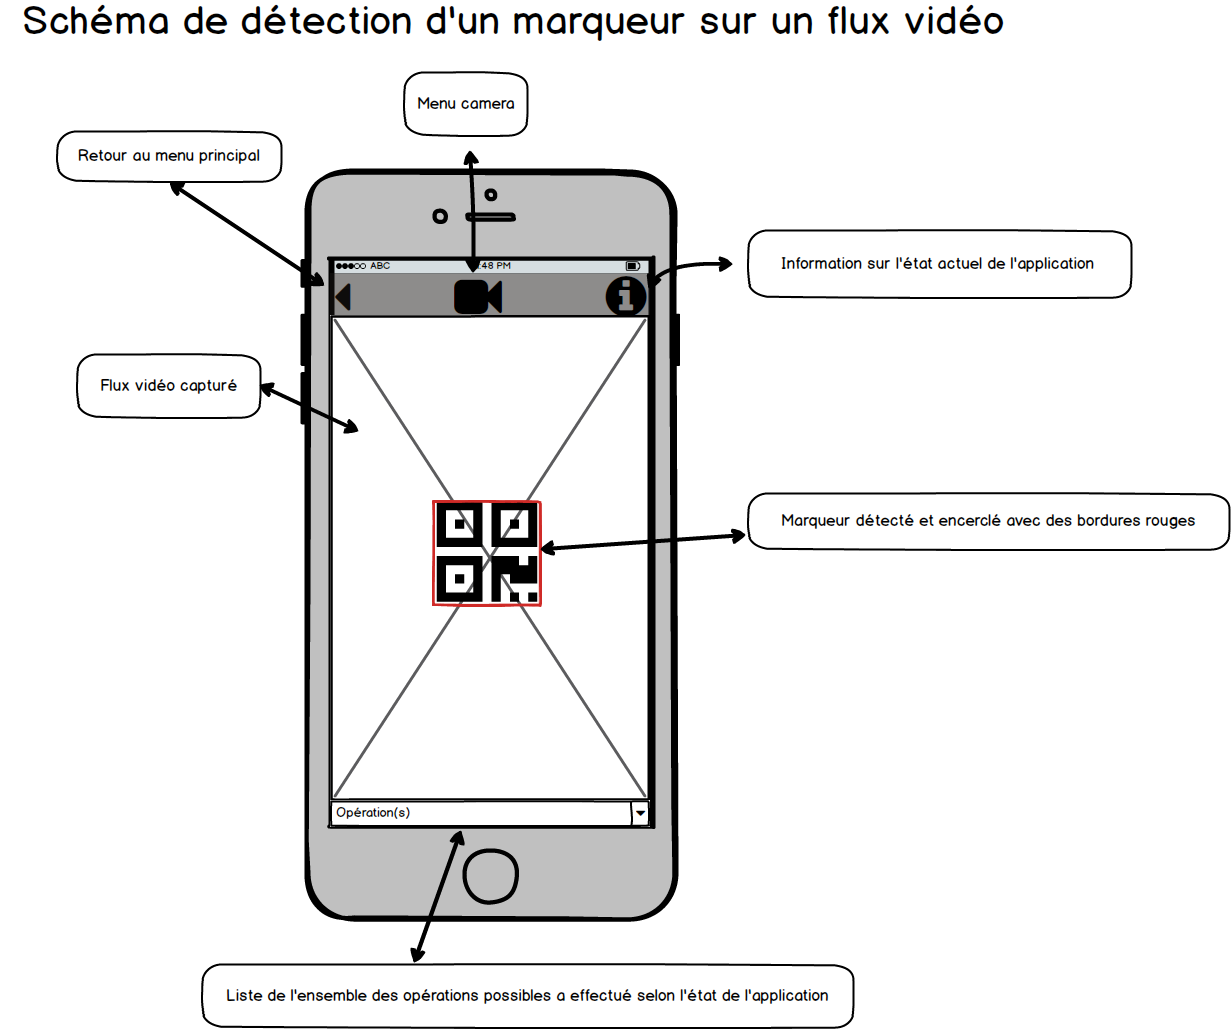
\includegraphics[width = 15cm,height=15cm]{prototype_app.png}
  \caption{Maquette de détection d'un marqueur sur un flux vidéo}
\end{figure}

%Accessibilité pour les personnes à mobilité réduite
\subsection{Accessibilité pour les personnes à mobilité réduite}
\begin{itemize}
\item Minimiser le nombre de boutons, un bouton pour accéder à l'interface spécifique à l'appareil cible, et un bouton pour la quitter.[Fort]
\item Les boutons doivent avoir les caractéristiques suivantes :[Moyen]
\begin{itemize}
\item Les boutons et les marqueurs "ArUco"(Cf.~\ref{label-aruco}) auxquels ils sont associés ont la même taille, pour que les boutons associés aux marqueurs ne se chevauchent pas si l'utilisateur s'en approche.

\item Les boutons des interfaces spécifiques ont des dimensions fixes (100 px, 100 px), la couleur de chaque bouton diffère de l'autre, tout dépend de l'action associée au bouton.

\item Les boutons sont sélectionnables graphiquement par un seul clic, pour des raisons de sécurité.
\end{itemize}
\item Par défaut, l'utilisateur, peut faire apparaître qu'une seule interface spécifique au marqueur, pour des raisons de sécurité. Mais il peut désactiver cette option dans les paramètres de l'application, afin de pouvoir apparaître plusieurs interfaces spécifiques à la fois au marqueurs présent dans le flux vidéo.[Moyen]
\end{itemize}

%Protocoles de communications et traitement de données
\subsection{Protocoles de communications et traitement de données}
\begin{itemize}
\item Envoyer l'identifiant récupéré à partir du marqueur "ArUco"(Cf.~\ref{label-aruco}) et l'identifiant en cours de sessions sur l'application au serveur via le protocole MQTT (Cf.\cite{Ref21}).[Critique]
\item Envoyer une demande d'information sur un marqueur "ArUco"(Cf.~\ref{label-aruco}) depuis l'application vers le serveur via le protocole MQTT .[Critique]
\item Récupérer des informations sur l'appareil à manipuler (son type et est-ce qu'on a le droit de le manipuler) à partir du serveur et via le protocole MQTT.[Critique]
\item Traiter une demande d'information concernant l'identifiant d'un marqueur "ArUco" depuis le serveur.[Critique]
\item Comparer le champ identifiant de chaque élément de la base de données avec l'identifiant recherché.[Critique]
\item Vérifier sur le serveur si la requête envoyer depuis le système est une requête valide en examinant ses champs.[Critique]
\item Effectuer une requête MQTT de type publish sur le Broker (protocole MQTT détaillé dans les choix d'implémentation) à fin d'y communiquer la requête demandée par le système et à effectuer sur l'appareil.[Critique]
\item Effectuer une requête MQTT de type subscribe depuis Raspberry PI(Cf.~\ref{label-raspberry}) sur le Broker afin d'y récupérer la requête demandée par le système.[Critique]
\item Exécuter la requête récupérée depuis le Broker sur le Raspberry PI, en extrayant les champs qu'elle contient et en exécutant la partie du code relatif à ces derniers.[Critique]
\end{itemize}

\begin{figure}[H]
  \centering
  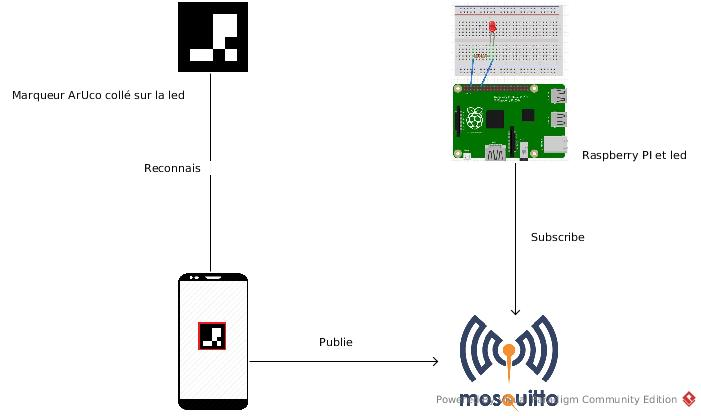
\includegraphics[width = 15cm,height=10cm]{maquette_finale.jpg}
  \caption{Prototype final du déploiement de l'application}
\end{figure}



%Besoins non fonctionnels
\section{Besoins non fonctionnels}

\subparagraph{Réactivité :} Le temps de reconnaissance d'un marqueur "ArUco"(Cf.~\ref{label-aruco}) ne doit pas dépasser 0.2 secondes, le temps nécessaire pour mener une action complète (voir cas d'utilisations) ne doit pas dépasser 2 secondes.
\par Appareils de tests utilisé : Samsung S6 Edge, Asus ZenFone 2 (ZE551ML), ordinateur portable Lenovo ThinkPad T440s, leurs caractéristiques sont indiquées dans la  ~\autoref{table1} : \par
\begin{table}[H]
\centering
\caption{Caractéristiques des appareils de tests}
\label{table1}
\begin{tabular}{|l|l|l|l|l}
\cline{1-4}
Camera       & Processeur                                                                                                     & système d'exploitation                                                 & Mémoire vif                                                      &  \\ \cline{1-4}
16 Megapixel & \begin{tabular}[c]{@{}l@{}}Exynos 7420 (64-bit, 14nm) \\ Octa core (2.1GHz Quad \\ + 1.5GHz Quad)\end{tabular} & \begin{tabular}[c]{@{}l@{}}Android : 6.0.1\\  Marshmallow\end{tabular} & \begin{tabular}[c]{@{}l@{}}RAM: 4GO RAM \\ (LPDDR4)\end{tabular} &  \\ \cline{1-4}
13 Megapixel & \begin{tabular}[c]{@{}l@{}}Intel Atom Z3580 (64-bit)\\  Quad-core 2.3 GHz\end{tabular}                         & \begin{tabular}[c]{@{}l@{}}Android : 6.0.1\\  Marshmallow\end{tabular} & \begin{tabular}[c]{@{}l@{}}RAM: 4GO RAM\\  (DDR3)\end{tabular}   &  \\ \cline{1-4}
HD 720p      & \begin{tabular}[c]{@{}l@{}}Intel® Core™ i7-4600U\\ 2.1 GHz, cache L3 4 Mo\end{tabular}                         & Ubuntu 16.04                                                           & \begin{tabular}[c]{@{}l@{}}RAM: 8GO RAM\\ (DDR3L)\end{tabular}   &  \\ \cline{1-4}
\end{tabular}
\end{table}

%\end{table}

\subparagraph{Test :}
Le test sera effectué sous forme de tableau, on additionne les deux premiers champs des tables suivantes ~\autoref{table2} et ~\autoref{table3}, le résultat ne doit pas dépassé 1 seconde.
\par
%Tableau comparatif des temps de traitements
\begin{table}[H]
\centering
\caption{Test de réactivité de l'application sur un ordinateur portable ThinkPad T440s}
\label{table2}
\begin{tabular}{lllll}
\cline{1-3}
\multicolumn{1}{|c|}{\begin{tabular}[c]{@{}c@{}}Temps de\\ reconnaissance ArUco\end{tabular}} & \multicolumn{1}{c|}{\begin{tabular}[c]{@{}c@{}}Temps d'échange\\ Application - Matériel\end{tabular}} &\multicolumn{1}{l|}{Temps total} &  &  \\ \cline{1-3}
\multicolumn{1}{|c|}{30-40 ms}                                                                & \multicolumn{1}{c|}{0,30-0,50 ms}                                                                       & \multicolumn{1}{c|}{30,50-40,50} &  &  \\ \cline{1-3}
                                                                                              &                                                                                                         &                                  &  &  \\
                                                                                              &                                                                                                         &                                  &  & 
\end{tabular}
\end{table}
\begin{table}[H]
\centering
\caption{Test de réactivité de l'application sur un Smartphone Samsung S6 Edge Plus}
\label{table3}
\begin{tabular}{lllll}
\cline{1-3}
\multicolumn{1}{|c|}{\begin{tabular}[c]{@{}c@{}}Temps de\\ reconnaissance ArUco\end{tabular}} & \multicolumn{1}{c|}{\begin{tabular}[c]{@{}c@{}}Temps d'échange\\ Application - Matériel\end{tabular}} & \multicolumn{1}{l|}{Temps total} &  &  \\ \cline{1-3}
\multicolumn{1}{|c|}{30-40 ms}                                                                & \multicolumn{1}{c|}{1-9 ms}                                                                           & \multicolumn{1}{c|}{39-49}       &  &  \\ \cline{1-3}
                                                                                              &                                                                                                       &                                  &  &  \\
                                                                                              &                                                                                                       &                                  &  & 
\end{tabular}
\end{table}
Le procédé de test sera expliqué dans la section Tests comportant les figures (Cf.~\ref{fig28}, ~\ref{fig29})

\subparagraph{Accessibilité pour l'interface:} L'application doit être relativement facile à manipuler afin de satisfaire les besoins des personnes à mobilité réduite (grands boutons ..).

\subparagraph{Test :} Le test sera proposé sous la forme d'un questionnaire, ce dernier sera distribué au futur utilisateur à mobilité réduite, les réponses du questionnaire serviront à une éventuelle refonte de l'interface.\par
\begin{enumerate}
  \item Que pensez-vous du positionnement boutons et des fenêtres ?
  \item Que pensez-vous de la taille des boutons, est-elle convenable à votre cas ? 
  \item Que pensez-vous de la lisibilité du texte ?
  \item La navigation entre les différentes fenêtres de l'application vous semble-t-elle aisée ?
  \item Est-ce que les sons réactifs, aux actions effectuées dans l'application vous sont bénéfiques ?
  \item Est-ce que les raccourcis claviers proposés par notre application vous semblent ils appropriés à vos besoins ?
  \item Est-ce que le temps nécessaire pour mener une action au complet (allumer une lampe par exemple) vous semble convenable ?
\end{enumerate}

%Contraintes
\section{Contraintes}

\begin{itemize}
  \item L'exécution intensive de l'application ne doit pas provoquer une utilisation gourmande au niveau des ressources de l'appareil utilisé, l'application ne doit pas accéder au plus de 2 GO de RAM (La capacité de RAM des appareils disposés pour les tests).
  \item Les plate-formes de développement  utilisées doivent être libre-service, sous licence GPL ou LGPL.
  \item La version minimale d'Android est la version 5.0, car le WebRTC est reconnu que depuis cette version ou plus.
  \item Définir un identifiant unique à chaque enregistrement pour maintenir l'intégrité de la base de données.
  \item Utilisation d'un fichier de stockage interne '.json' qui fait office de base de données.
  \item Les fichiers temporaires seront supprimés après la fermeture de l'application, l'ensemble des données stockées sur l'appareil ne doivent pas dépasser 2 GO.
\end{itemize}

%Diagramme de Gantt
\section{Diagramme de Gantt}
\begin{sidewaysfigure}
\begin{center}

\definecolor{barblue}{RGB}{153,204,254}
\definecolor{groupblue}{RGB}{51,102,254}
\definecolor{linkred}{RGB}{165,0,33}
\renewcommand\sfdefault{phv}
\renewcommand\mddefault{mc}
\renewcommand\bfdefault{bc}
\setganttlinklabel{s-s}{START-TO-START}
\setganttlinklabel{f-s}{FINISH-TO-START}
\setganttlinklabel{f-f}{FINISH-TO-FINISH}
\sffamily

\begin{ganttchart}[hgrid,vgrid, y unit chart=0.7cm]{1}{24}
\gantttitle{Semaines}{24}\\
\gantttitlelist{1,...,12}{2}\\
\ganttbar[bar/.style={fill=green}]{Bibliographie}{1}{3}\\
\ganttgroup{Analyse des besoins}{1}{1}\\

\ganttgroup{Traitement d’image}{1}{12}\\
\ganttbar[bar/.style={fill=green}]{Récupérer le flux vidéo d'une caméra}{3}{5}\\
\ganttbar[bar/.style={fill=green}]{Identifier la présence des marqueurs ArUco dans un flux vidéo}{6}{7}\\
\ganttbar[bar/.style={fill=green}]{Encadrer les bords de chaque marqueur ArUco existant}{8}{9}\\
\ganttbar[bar/.style={fill=green}]{Transformer les marqueurs encadrés précédemment en bouton}{10}{12}\\
\ganttlink[link type=f-s]{elem3}{elem4}
\ganttlink[link type=f-s]{elem4}{elem5}
\ganttlink[link type=f-s]{elem5}{elem6}

\ganttgroup{Interface homme-machine}{13}{18}\\
\ganttbar[bar/.style={fill=red}]{Associer une étiquette à chaque marqueur présent dans le flux vidéo}{13}{13}\\
\ganttbar[bar/.style={fill=red}]{Sélectionner graphiquement un des marqueurs présent dans le flux vidéo}{13}{13}\\
\ganttbar[bar/.style={fill=red}]{Associer une interface spécifique au marqueur sélectionné}{14}{15}\\
\ganttbar[bar/.style={fill=red}]{Faire apparaître les traitements possibles dans un menu}{15}{15}\\
\ganttbar[bar/.style={fill=red}]{Envoyer au serveur les informations sur la sélection de l’utilisateur}{16}{16}\\
\ganttbar[bar/.style={fill=red}]{Mettre à jour le menu à chaque changement d’état de l’appareil}{17}{17}\\
\ganttbar[bar/.style={fill=red}]{Quitter l’interface en cliquant sur un bouton configurable}{18}{18}\\
\ganttlink[link type=s-s]{elem8}{elem9}
\ganttlink[link type=s-s]{elem10}{elem11}
\ganttlink[link type=f-s]{elem11}{elem12}
\ganttlink[link type=f-s]{elem12}{elem13}
\ganttlink[link type=f-s]{elem13}{elem14}
\ganttlink[link type=f-s]{elem9}{elem10}
\ganttlink[link type=f-s]{elem6}{elem7}


\ganttgroup{Protocoles de communications et traitement de données}{19}{24}\\
\ganttbar [bar/.style={fill=red}]{Envoyer l’identifiant  du marqueur ArUco au serveur}{19}{19}\\
\ganttbar[bar/.style={fill=red}]{Traiter la requête au niveau du serveur et l'envoyer au Rraspberryaspberry PI}{20}{21}\\
\ganttbar[bar/.style={fill=red}]{L'exécution de l'ordre par le Raspberry PI}{22}{24}\\
\ganttlink[link type=f-s]{elem14}{elem15}
\ganttlink[link type=f-s]{elem16}{elem17}
\ganttlink[link type=f-s]{elem17}{elem18}


\end{ganttchart}
\caption{DIagramme de Gantt.}
\end{center}
\end{sidewaysfigure}

\newpage

%Architecture logicielle
\section{Architecture logicielle}
%Introduction
\subsection{Introduction}
Dans cette partie, nous présenterons l'architecture de notre logiciel, modélisé via le langage unifié UML, en schématisant tout d'abord nos cas d'utilisation par des diagrammes de cas d'utilisation, puis nous détaillerons le séquencement de notre application, en décrivant chaque acteur, le rôle qu'il interprète, et le déroulement des actions effectuées dans une ligne de temps.\par
Nous présenterons ensuite les différentes classes de notre diagramme de classe, les méthodes et attributs qu'elles contiennent, ainsi que les relations existantes entre elles.\par
Et pour finir, nous expliquerons comment notre application est déployée, ce qui permettra de bien assimiler l'interaction de notre logiciel avec les différents composants matériels.\par
%Cas d'utilisation
\subsection{Cas d'utilisations}
Dans cette partie, nous avons énoncé le cas d'utilisation le plus basique de notre application, il s'agit de la manipulation d'une lampe via cette dernière.\par
Pour les autres cas d'utilisation, se référer aux annexes.
\subsubsection{Cas d'une lampe}
\begin{itemize}
  \item L'utilisateur pointe sa tablette sur un marqueur ArUco.
  \item Le système détecte le code ArUco et y affiche un bouton d'activation. 
  \item L'utilisateur sélectionne le code ArUco en cliquant sur le bouton spécifique.
  \item Le système affiche une interface spécifique à la lampe.
  \item L'utilisateur demande d'éteindre ou d'allumer la lampe via l'application.
  \item Le système envoie la requête au serveur web.
  \item Le serveur traite la requête et l'envoie au Raspberry PI.
  \item Le Raspberry PI exécute l'ordre et allume donc ou éteint la lampe.
\end{itemize}
  \newpage
\begin{figure}[!ht]
  \centering
  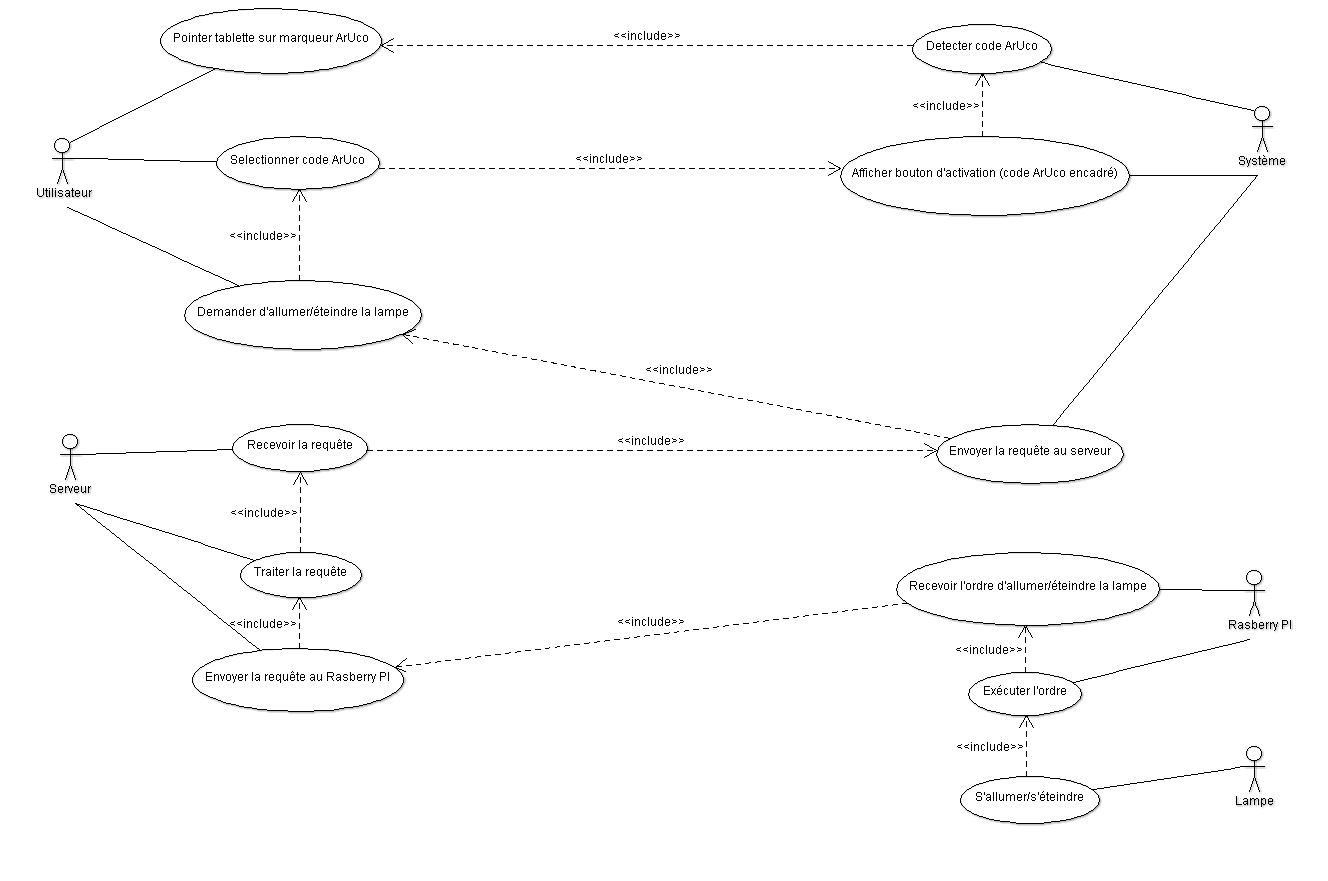
\includegraphics[width = 15cm,height=21cm]{DCU_Lampe.png}
  \caption{Diagramme de cas d'utilisations d'une lampe}
\end{figure}
%Digrammes de séquences
\subsection{Diagrammes de séquences}
\subsubsection{Cas d'une lampe}
\begin{enumerate}
\item Tout d'abord, l'utilisateur pointe son appareil sur un ou plusieurs codes ArUco, c'est l'application qui se charge de récupérer le flux vidéo et de le traiter.
	\begin{enumerate}
	\item L'application détecte le ou les codes ArUco, un bouton cliquable est affiché sur le code ArUco dans le flux vidéo.
	\end{enumerate}
\item L'utilisateur sélectionne un code ArUco en cliquant sur un des boutons afficher.
	\begin{enumerate}
	\item l'application vérifie que le code ArUco est bien reconnu, en extrayant la valeur contenue dans le code, et en la comparant aux valeurs contenues dans un fichier .json faisant office de base de données. 
	\end{enumerate}
\item Si le code a bien été reconnu.
	\begin{enumerate}
	\item l'application affiche une interface spécifique à l'appareil identifié par ce code.
	\end{enumerate}
\item L'utilisateur demande d'allumer ou d'éteindre la lampe via l'application.
	\begin{enumerate}
	\item L'application envoie la requête au serveur "Broker"(Cf.\cite{Ref32}).
	\end{enumerate}
\item Le Raspberry PI récupéré la requête depuis le "Broker".%THERE
\item Le Raspberry PI exécute l'ordre et allume ou éteint la lampe.
\item L'application met à jour l'interface graphique selon l'état actuel de la lampe.
\end{enumerate}
\newpage
\begin{figure}[!ht]
  \centering
  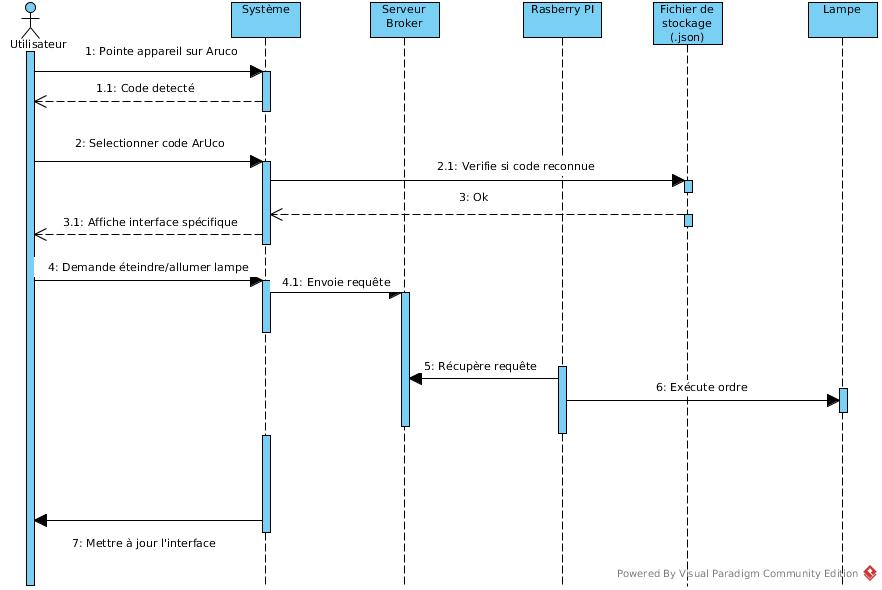
\includegraphics[width = 15cm,height=20cm]{DDS_Lampe.jpg}
  \caption{Diagrammes de séquences d'une lampe}
\end{figure}
\newpage
%Digramme de classe
\subsection{Diagramme de classe}
\begin{figure}[!ht]
  \centering
  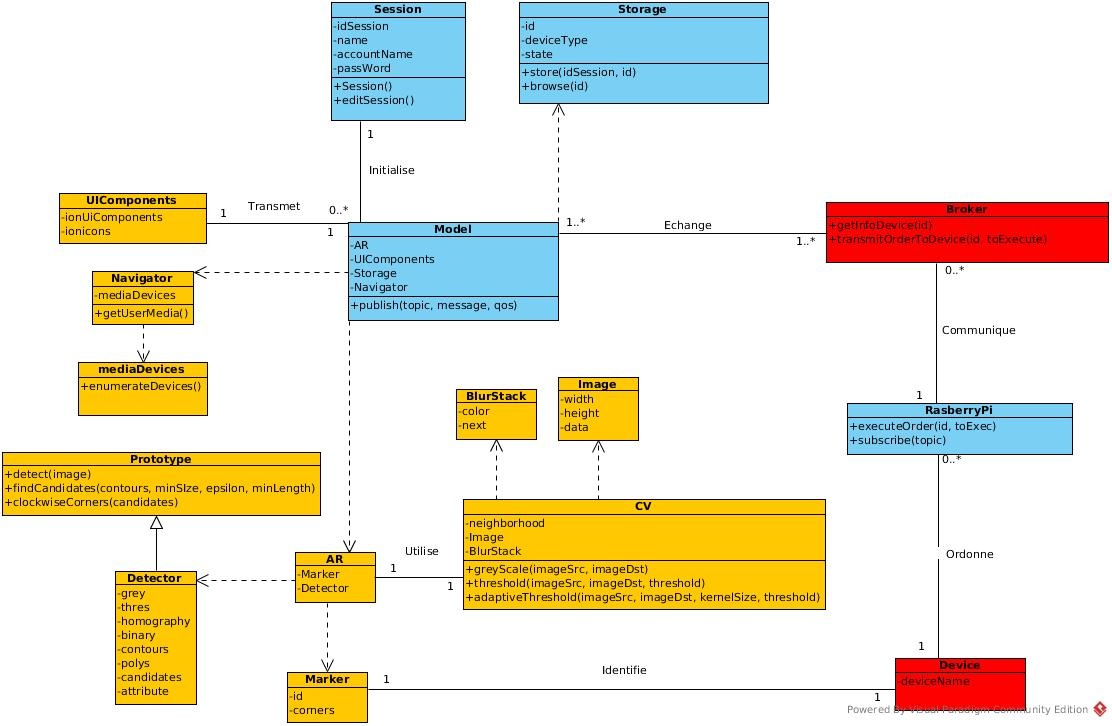
\includegraphics[width = 15cm,height=20cm]{DDC_C.jpg}
  \caption{Diagramme de classe,
  Bleu : les classes que nous proposons, 
  Rouge : classes qui modélisent des entités déjà existantes, 
  Jaune : les classes que nous avons reprises. 
  }
\end{figure}
\newpage
\par
Afin de réaliser notre projet, nous avons repris la classe 'AR' qui se charge du traitement de la réalité augmentée ainsi que la classe 'CV' utilisée par 'AR'.\par
La couleur jaune symbolise les classes qu'on a repris.\par
La couleur rouge, quant à elle, symbolise des entités physiques, 'Device' étant un appareil à manipuler (par exemple; une lampe), 'Broker' est un serveur préexistant et implémenté qui sert de passerelle de communication entre l'application et le Raspberry PI.\par 
\subsubsection{Les classes}
\subparagraph{Navigator}
La classe 'Navigator' est une API web qu'on a utilisée afin de réaliser notre projet, cette classe nous permet entre autres de récupérer le flux vidéo de la caméra via la méthode 'getUserMedia()'.\par
\subparagraph{UIComponents}
La classe 'UIComponents' contient l'ensemble des composants graphiques fournis par Ionic, un framework open-source permettant de créer des applications mobiles, les méthodes contenues dans cette classe nous permettent de tracer l'interface graphique de notre application.\par
\subparagraph{Model}
La classe principale de notre application est 'Model',elle symbolise le modèle, cette classe contient une instance de chaque une des classes : 'Navigator', 'AR' et 'Storage', ceci est donc représenté dans le diagramme de classe par une relation de dépendance entre 'Model' et ces classes.\par%THERE
Le modèle peut échanger une requête avec le broker afin de changer l'état d'un appareil 'Device', lui demander de récupérer l'état courant d'un appareil, vice versa, le serveur peut lui transmettre l'état courant d'un appareil et l'informer que l'état de l'appareil a changé.\par
Afin d'accéder à l'application l'utilisateur aura besoin de s'authentifier, plusieurs sessions peuvent subsister dans l'application alors qu'une session ne peut appartenir qu'à un seul modèle, c'est ce qui va permettre à un utilisateur d'avoir le droit de modifier l'état courant d'un appareil, à chaque session sont attribués un nombre d'appareils.\par
Entre 'Model' et 'UIComponents' subsiste une relation un à un, elle permet au modèle de transmettre des données à 'UIComponents' afin que l'affichage graphique de l'application change selon ces données.\par
\subparagraph{Storage}
La classe 'Storage' fait office de base de données, c'est là que nous stockerons l'identifiant, le type et l'état de chaque appareil manipulé par l'application, et avant qu'un utilisateur puisse manipuler un appareil identifié par un code ArUco, on s'assurera de son existence dans l'instanciation de cette classe.\par
\subparagraph{Session}
C'est dans la classe 'Session' qu'on stock les sessions existantes dans l'application, il faudra enregistrer toutes les sessions existantes dans un fichier '.json'.\par 
\subparagraph{Broker}
Cette classe modélise le serveur Broker qui servira de passerelle entre l'application et le Raspberry PI, cette entité se chargera essentiellement de recevoir des requêtes depuis l'application afin que le Raspberry PI puisse  les récupérer.\par
Le serveur Broker peut communiquer avec plusieurs Raspberry PI, un Raspberry PI ne reçoit de requête que de la part d'un seul serveur, cette relation permet au Raspberry PI de récupérer des requêtes depuis le serveur.
\subparagraph{Raspberry PI}
Elle modélise le Raspberry PI, qui se chargera d'exécuter l'ordre du serveur web et de lui envoyer un acquittement après traitement de cette requête.\par%THERE
Le Raspberry PI a besoin de communiquer des ordres à un ou plusieurs appareils, un appareil ne reçoit d'ordre que de la part d'un seul Raspberry PI.
\subparagraph{Device}
L'appareil manipulé et identifié par un code ArUco est modélisé par 'Device', il contient un libellé et est relié au Raspberry PI afin qu'ils puissent communiquer.\par
La classe 'Marker' existait dans le code qu'on a repris et qui nous permet de générer de la réalité augmentée, elle contient l'identifiant du code reconnu en cours de traitement, cet identifiant correspond à l'appareil manipulé et modélisé par 'Device', à chaque 'Marker' correspond un unique 'Device' et vice versa.\par
Pour ce qui est des classes jaunes, il n'y a que quelques liens entre elles qui nous intéressent, tels que le fait que la classe 'AR', qui permet de reconnaître des codes ArUco, utilise la classe 'CV', qui est basée sur OpenCV (Cf.\cite{Ref9}), la classe 'AR' contient une classe 'Marker', qui modélise le marqueur ArUco, elle contient un attribut 'id' qui nous intéresse et qui permet d'identifier un appareil modélisé par 'Device', c'est pour cela qu'entre la classe 'Marker' et la classe 'Device' réside une relation 1 à 1.  
\newpage

%Diagramme de déploiement
\subsection{Diagramme de déploiement}
\begin{figure}[!ht]
  \centering
  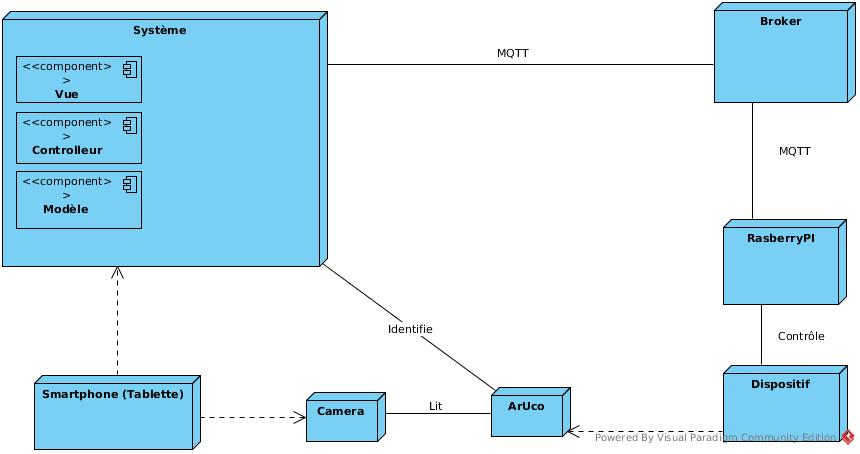
\includegraphics[width = 15cm,height=20cm]{DDep.jpg}
  \caption{Diagramme de déploiement}
\end{figure}
\newpage
\par
L'objet 'Système' modélise notre application au complet, elle contient une vue, un contrôleur et un modèle.\par
Les connexions entre le système, le serveur web, le Raspberry PI et le dispositif se font via le protocole MQTT(Cf.\cite{Ref21}).\par
Le système est installé dans le smartphone (ou la tablette) de l'utilisateur, qui est donc équipé d'une caméra et qui permet de capturer un flux vidéo afin de scanner d'éventuels codes ArUco.\par
Ces codes ArUco permettent d'identifier des dispositifs.

%Implémentation
\section{Implémentation}

%Choix téchniques

%Marqueur ArUco
\subsubsection{Marqueurs ArUco :}

\begin{figure}[h!]
  \centering
  \label{label-aruco}
  
\includegraphics[width = 5cm,height=5cm]{ArucoMarker.jpg}
  \caption{Marqueur AruCo}
  \href{url}{http://muro.ucsd.edu/img/ArucoMarker.jpg} 
  
\end{figure}

"An ArUco marker is a synthetic square marker composed by a wide black border and a inner binary matrix which determines its identifier (id). The black border facilitates its fast detection in the image and the binary codification allows its identification and the application of error detection and correction techniques. The marker size determines the size of the internal matrix. For instance a marker size of 4x4 is composed by 16 bits."(Cf.\cite{ref16}).

%Application mobile
\subsubsection{Application mobile}
Nous avons choisi de développer une application web, car la gestion des interfaces est plus facile avec le \texttt{HTML5 et CSS3}, et aussi pour assurer l'extensibilité de l'application, comme ça notre application peut être exécutée dans plusieurs plateformes. Donc nous avons décidé de développer notre application sous les framworks Ionic et Cordova, pour des raisons que nous allons expliquer en dessous. la figure 9: montre les logos de ces téchnologies.
\begin{figure}[h!]
\centering
	
\includegraphics[width = 16cm,height=8cm]{cordova-ng-ionic.png}
    \caption{Les framework de développement. \href{url}{http://coenraets.org/blog/wp-content/uploads/2014/06/cordova-ng-ionic.png}} 
	\label{label-ionic}
\end{figure}

%Ionic framework
\subsubsection*{Ionic framework :}
Ionic Framework est un mélange d’outils et de technologies pour développer des applications mobiles hybrides rapidement et facilement. Il s’appuie sur AngularJS pour la partie application web du framework et sur Cordova  pour la partie construction des applications natives. Ce framework open source permet de développer une application déployable sur plusieurs environnements tel qu’un site web ou une application mobile pour des systèmes tel que Android ou iOS ou Windows Phone…(Cf.\cite{Ref19})\par 
Nous avons choisi la plateforme Ionic car il est compatible avec la bibliothèque pour la reconnaissance des codes ArUco, citée auparavant. Ionic propose le design pattern "MVC'" prêt à l'emploi, permettant de factoriser le code, et de répartir les différentes parties du code selon ses fonctionnalités.

%AngularJS :
\subsubsection*{AngularJS :}
AngularJS4 est le framework JavaScript libre et open-source5 développé par Google.
AngularJS est fondé sur l’extension du langage HTML par de nouvelles balises (tags) et attributs pour aboutir à une définition déclarative des pages web, par opposition à l’utilisation systématique de l’élément "div" et à la définition des éléments de présentation en JavaScript.(Cf.\cite{ref33})

%Cordova
\subsubsection*{Cordova :}
Apache Cordova est un framework de développement mobile open-source. Il permet d'exploiter les technologies Web courantes telles que HTML5, CSS3 et JavaScript pour développer des applications multi-plateformes, évitant ainsi l'utilisation des langages natifs propres aux différentes plates-formes mobiles. Les applications s'exécutent dans des wrappers ciblés pour chaque plate-forme, elles s'appuient sur des API conformes aux standards permettant l'accès aux capteurs de chaque appareil, aux données ainsi qu'à l'état du réseau.(Cf.\cite{Ref34})

%Matériel et protocole de communication
\subsubsection{Matériel et protocole de communication}
\begin{figure}[ht]
\centering
    
\includegraphics[width = 15cm,height=3cm]{mosqutto.jpg}
    \caption {Protocoles de communication.\href{url}{https://oshlab.com/install-mqtt-mosquitto-raspberry-pi/}} 
	\label{label-image1}
\end{figure}

%Raspberry pi
\subsubsection*{Raspberry pi }
\par
\begin{figure}[ht]
\centering
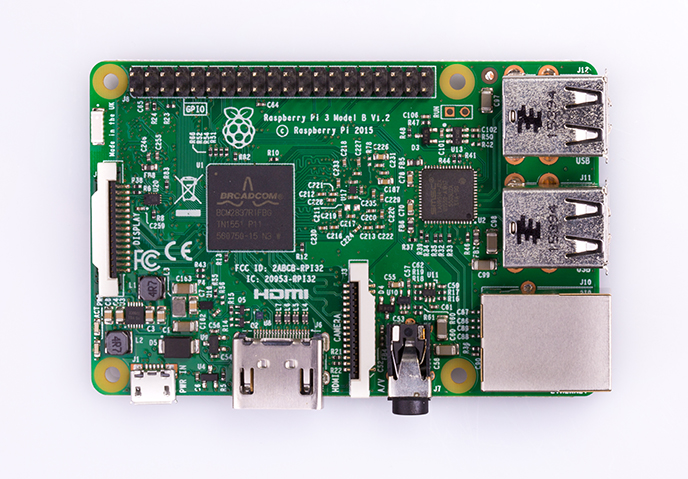
\includegraphics[width = 12cm,height=5cm]{rasberry.jpg}
 \caption {Raspberry Pi.\href{url}{https://www.raspberrypi.org/weekly/connected/}} 
	\label{label-raspberry}
\end{figure}
Le Raspberry pi est un nano ordinateur de la taille d'une carte de crédit que l'on peut brancher à un écran et utiliser comme un ordinateur standard. Sa petite taille, et son prix intéressant fait du Raspberry pi un produit idéal pour tester différentes choses, et notamment la création d'un serveur Web chez soi. Évidemment, pour sa taille il ne faut pas s'attendre à des performances incroyables, mais pour mettre en ligne des projets à montrer au client ou expérimenter avec linux c'est largement suffisant.(Cf.\cite{Ref20})
\subsubsection*{Mosquitto}
Mosquitto est un serveur MQTT Open Source (Broker) que l’on peut installer sur un Raspberry Pi (mais également sur d’autres plateformes) pour faciliter la communication entre objets connectés (M2M). Mosquitto est un outil idéal pour intégrer des objets connectés à un serveur domotique(Cf.\cite{ref29}).
\subsubsection*{MQTT}
MQTT permet concrètement aux appareils d'envoyer des informations sur un sujet donné à un serveur qui fonctionne comme un broker de messages. Le broker pousse ces informations vers les clients qui se sont précédemment abonnés (Cf.\cite{Ref21}).

%PAHO
\subsubsection*{PAHO}
"The Eclipse Paho project provides open-source client implementations of MQTT and MQTT-SN messaging protocols aimed at new, existing, and emerging applications for the Internet of Things (IoT)" (Cf.\cite{Ref28}).\par
PAHO est une implémentation du protocole MQTT disponible sous plusieurs langages de programmation, pour la réalisation de notre projet, nous avons utilisé les versions Python et Javascript de ce dernier.

%BROKER
\subsubsection*{Broker}
Une bonne définition en anglais de ce qu'est un "Broker" peut-être trouvé dans le lien cité ci-dessous. \par
"The counterpart to a MQTT client is the MQTT broker, which is the heart of any publish/subscribe protocol. Depending on the concrete implementation, a broker can handle up to thousands of concurrently connected MQTT clients. The broker is primarily responsible for receiving all messages, filtering them, decide who is interested in it and then sending the message to all subscribed clients. It also holds the session of all persisted clients including subscriptions and missed messages (More details). Another responsibility of the broker is the authentication and authorization of clients. And at most of the times a broker is also extensible, which allows to easily integrate custom authentication, authorization and integration into backend systems. Especially the integration is an important aspect, because often the broker is the component, which is directly exposed on the internet and handles a lot of clients and then passes messages along to downstream analyzing and processing systems. As we described in one of our early blog post subscribing to all message is not really an option. All in all the broker is the central hub, which every message needs to pass. Therefore it is important, that it is highly scalable, integratable into backend systems, easy to monitor and of course failure-resistant. For example HiveMQ solves this challenges by using state-of-the-art event driven network processing, an open plugin system and standard providers for monitoring." (Cf.\cite{Ref32}).\par
Un Broker, est donc le côté serveur de MQTT, il sert de passerelle entre plusieurs entités communiquant à travers le protocole MQTT.\par
Quelqu'un publie son message dans le Broker afin qu'un autre vient le récupérer.
%Frame et applications pour test
\subsection{Plate-formes et applications pour les tests}
\subsubsection*{GameBench}
GameBench est une application composée d'un ensemble d'outils pour Android et IOS permettant d'analyser efficacement le comportement d'une application et d'identifier les buggs générés par cette dernière(Cf.\cite{Ref30}).

%Code
\subsection{Code}

%Traitement d'image
\subsubsection{Traitement d'image}
Afin de récupérer le flux vidéo et le découper en images, pour ensuite les traiter et les analyser de sorte à détecter les marqueurs ArUco, nous avons récupéré le travail de \texttt{Juan Mellado} "la bibliothèque JS-ArUco"(Cf.\cite{Ref4}) qui se base sur \texttt{OpenCV}, avec une licence BSD(licence libre), tout en gardant ses droits.

%Récuperation du flux video
\subsubsection*{Récupération du flux vidéo}

	Dans cette partie nous avons commencé par adapter les dimensions du flux vidéo au matériel supportant l'application. Pour cela nous affichons le flux vidéo en plein écran, cela s'effectue, au niveau de la variable canvas : 
\medskip
\begin{lstlisting}
canvas.width = parseInt(window.screen.width);
canvas.height = parseInt(window.screen.height);
\end{lstlisting}

	Nous avons ensuite listé les IDs (identifiants) des caméras disponibles sur l'appareil dans un tableau, afin de passer l'identifiant de la caméra arrière en paramètre de la fonction \texttt{navigator.mediadevices GetUserMedia()}. Cela permet d'utiliser par défaut la caméra arrière pour récupérer le flux vidéo.
\begin{lstlisting}
.then(devices => {
      ...
      devices.forEach(function(device) {
        console.log(device.kind + ": " + device.label +
          " id = " + device.deviceId);
        // If the kind of the media resource is video, 
        if (device.kind == "videoinput") {  
          //  then we save it on the array videoDevices.
          videoDevices[videoDeviceIndex++] =  device.deviceId;    
        }
      });
      // Here we specified which camera we start,
      //  videoDevices[0] : Front Camera
      //  videoDevices[1] : Back Camera 
      constraints = { deviceId: { exact: videoDevices[1]  } };
    return navigator.mediaDevices.getUserMedia({ video: constraints });

\end{lstlisting}

%Traitement de vidéo et identification du marqueur ArUco
\subsubsection*{Traitement vidéo et identification de marqueur ArUco}

	Afin d'identifier la présence d'un marqueur ArUco, nous avons commencé par décomposer le flux vidéo en images individuelles via la fonction \texttt{snapshot()}.
\begin{lstlisting}
function snapshot(){
  context.drawImage(video, 0, 0, canvas.width, canvas.height);
  snappedImage = context.getImageData(0, 0, canvas.width, canvas.height); 
}
\end{lstlisting}

	La détection d'un marqueur ArUco se fait via la fonction \texttt{detectArUcoMarkers()} qui récupère les images capturées 'snappedImage' à l'aide de la fonction \texttt{snapshot()}, ces images sont passer à la fonction fournie par la bibliothèque JS-ArUco \texttt{arucoDetector.detect(snappedImage)} , celle-ci analyse les images et renvoie un tableau '\textit{markers}'  contenant tous les marqueurs détectés dans le flux vidéo et enfin on identifie le marqueur ArUco. 
\begin{lstlisting}
function detectArUcoMarkers(){
  	...
    	var markers = arucoDetector.detect(snappedImage);
  	...
}
\end{lstlisting}
\par
   Afin d'encadrer les marqueurs détectés par un rectangle rouge, on a eu recours à la fonction fournie par la bibliothèque JS-ArUco \texttt{draw Corners(markers)}, pour  étiqueter les marqueurs, la fonction \texttt{drawId(markers)} est appelée.
\begin{lstlisting}
function detectArUcoMarkers(){
	...
    drawCorners(markers);
    drawId(markers);
    ...
}
\end{lstlisting}

Des modifications ont été apportées à la fonction "\texttt{draw Id(markers)}", pour qu'on puisse associer une interface spécifique à chaque marqueur reconnu, ces modifications seront détaillées dans la section suivante.

%Interface Homme-machine
\subsubsection{Interface Homme-machine}
	Suite à la détection et l'identification du marqueur ArUco, nous avons abordé  l'implémentation de l'interface graphique afin de pouvoir interagir avec les appareils externes, pour réaliser cette tâche, nous avons modifié le code de la fonction "\texttt{draw Id(markers)}", en introduisant deux variables "\texttt{x Max ,y Max}", qui servent à redimensionner l'interface, en prenant comme repère les dimensions du marqueur ArUco, ensuite on applique un "\texttt{switch()}' sur les marqueurs détectés dans le flux vidéo, pour associer une interface spécifique sur le marqueur associé,  à l'aide de la fonction "\texttt{show Interface(x,x Max ,y,y Max ,interface Id ,ArUcoButtonId)}", une sorte de base de données locale.
\begin{lstlisting}
function drawId(markers){
  ...
  var xMax,yMax;
  for (j = 0; j !== corners.length; ++ j){
      ...
      //  [Begin CHANGED]
      xMax = Math.max(x, corner.x);
      yMax = Math.max(y, corner.y);
      ...
      switch(markers[i].id) {
          case 10:
              showInterface(x,xMax,y,yMax,"lampDiv","lampButton");
              break;
          case 100:
              showInterface(x,xMax,y,yMax,"shutterDiv","shutterButton");
              break;
          case 1000:
              showInterface(x,xMax,y,yMax,"doorDiv","doorButton");
              break;
          default:
              // Nothing
      }
	...
}
\end{lstlisting}

La fonction "\texttt{show Interface()}" affiche en premier lieu une interface "\texttt{ balise HTML}" qui contiendra le boutton "\texttt{ArUcoButton }" au-dessus du marqueur portant le libellé de l'appareil associé, et ayant les mêmes coordonnées et dimensions que celles du marqueur (C.f~\ref{ihm1}), ainsi si on clique sur "\texttt{ArUcoButton }" la fonction "\texttt{showSpecified-
Interface(ArUcoButtonId, SpecifiedInterfaceId)}' est exécutée, cela permet de basculer vers l'interface contenant les ordres à envoyer au serveur pour manipuler le matériel.
\begin{lstlisting}
function showInterface(x,xMax,y,yMax,interfaceId,ArUcoButtonId){
	var lampInterface = document.getElementById(interfaceId);
	lampInterface.style.left = x + "px";
	lampInterface.style.top = y + "px";
	...
	showArUcoButton(x,xMax,y,yMax,ArUcoButtonId);
	...
    }
\end{lstlisting}
  
 Après la sélection du marqueur, une interface graphique spécifique (contenant les différentes opérations proposées par notre application) apparaît( Cf.Figure ~\ref{ihm2}), selon l'identifiant du marqueur choisi, dans le but d'interagir avec l'appareil externe qui lui correspond :
\begin{lstlisting}
function showSpecifiedInterface(ArUcoButtonId,SpecifiedInterfaceId){
	...
	lampInterface.style.display = "inline";
	hideArUcoButton(ArUcoButtonId);
	...
}

\end{lstlisting}

	Pour finir, l'application envoie une requête contenant l'action choisie par l'utilisateur auparavant  et l'identifiant du marqueur à un serveur, le Raspberry PI y récupère ces informations et exécute l'ordre de l'utilisateur, Cette partie sera détaillée d'avantage dans la section \texttt{Protocoles de communications et traitement de données} qui va suivre.
    
%Réalisation
\subsubsection{Réalisation } 
\begin{itemize}
\item Identification de marqueurs ArUco :
Cette figure (Cf.Figure ~\ref{ihm1}) illustre la procédure d'identification et de reconnaissance de codes ArUco par notre application et ceci en temps réel, des boutons libellés au nom des appareils reconnus selon leurs identifiants apparaissent sur les marqueurs ArUco, si un marqueur ArUco n'a pas été reconnu (son identifiant n'est pas référencé dans l'application), il est juste encadré par un rectangle rouge et son contenu est affiché en haut en bleu. 
\begin{figure}[H]
  \centering
   \label{ihm1}
    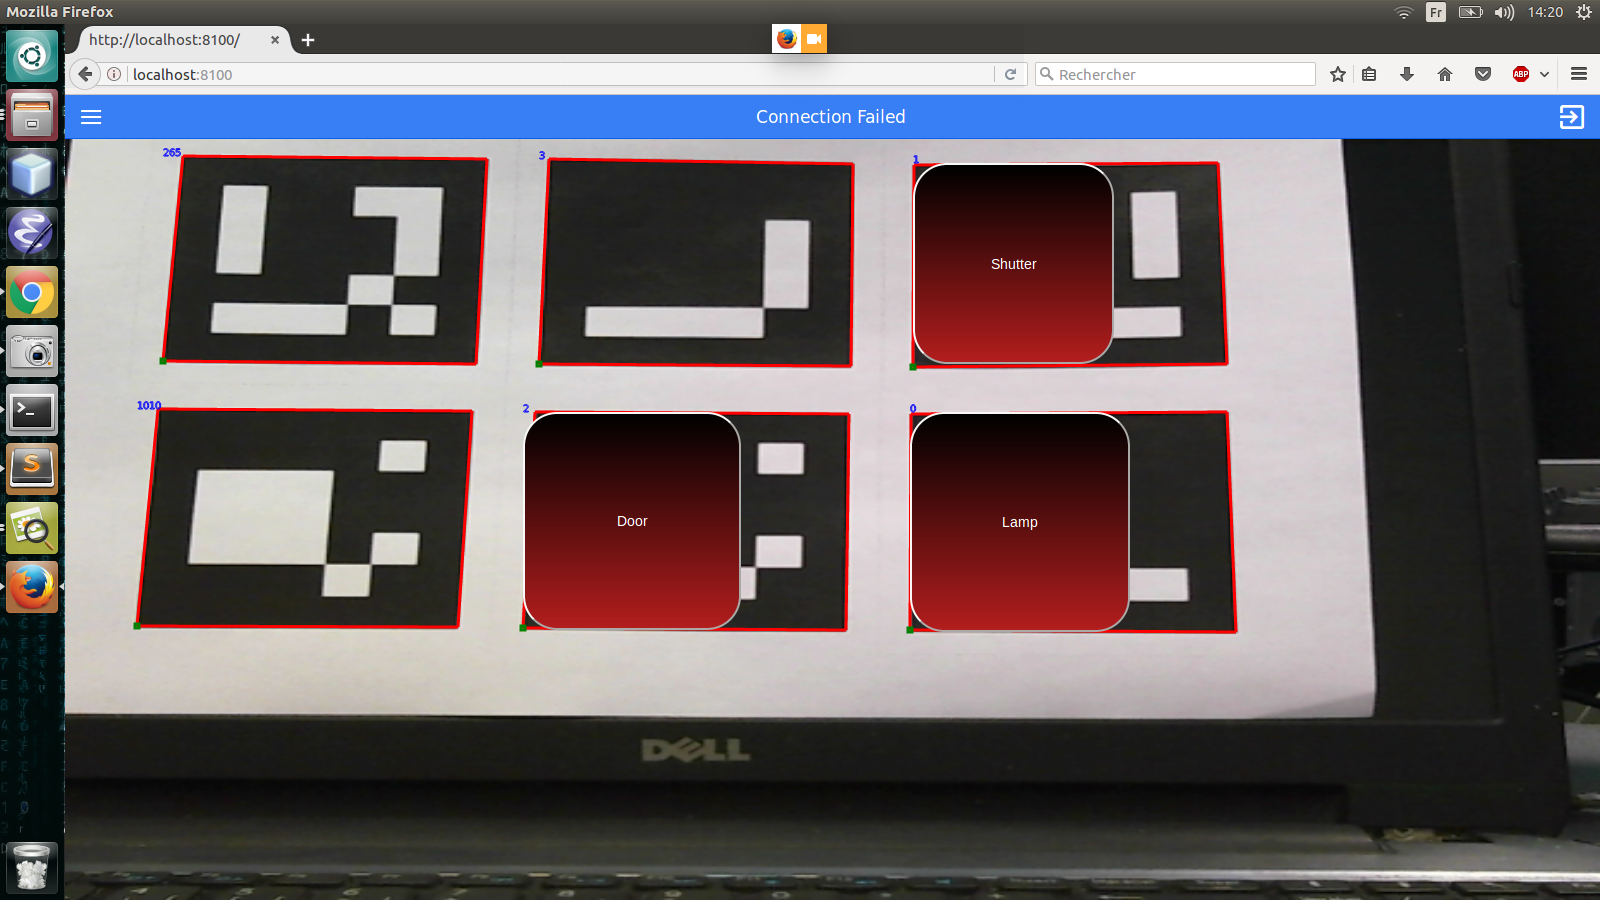
\includegraphics[width = 11cm,height=8cm]{3.png}
     \caption{Identification des marqueurs "ArUco"}
\end{figure}
\end{itemize}

\begin{itemize}

\item Interface Homme-machine :
Dans le but de paramétrer notre IHM, nous avons décidé d'ajouter un menu de paramétrage "\texttt{Setting}" qui contient 3 boutons pour pouvoir :
\begin{itemize}
\item Donner la possibilité de gérer plusieurs interfaces à la fois, par défaut l'application nous permet d'afficher une seule interface au cas où plusieurs marqueurs sont affichés sur le flux vidéo.
\begin{figure}[H]
  \centering
    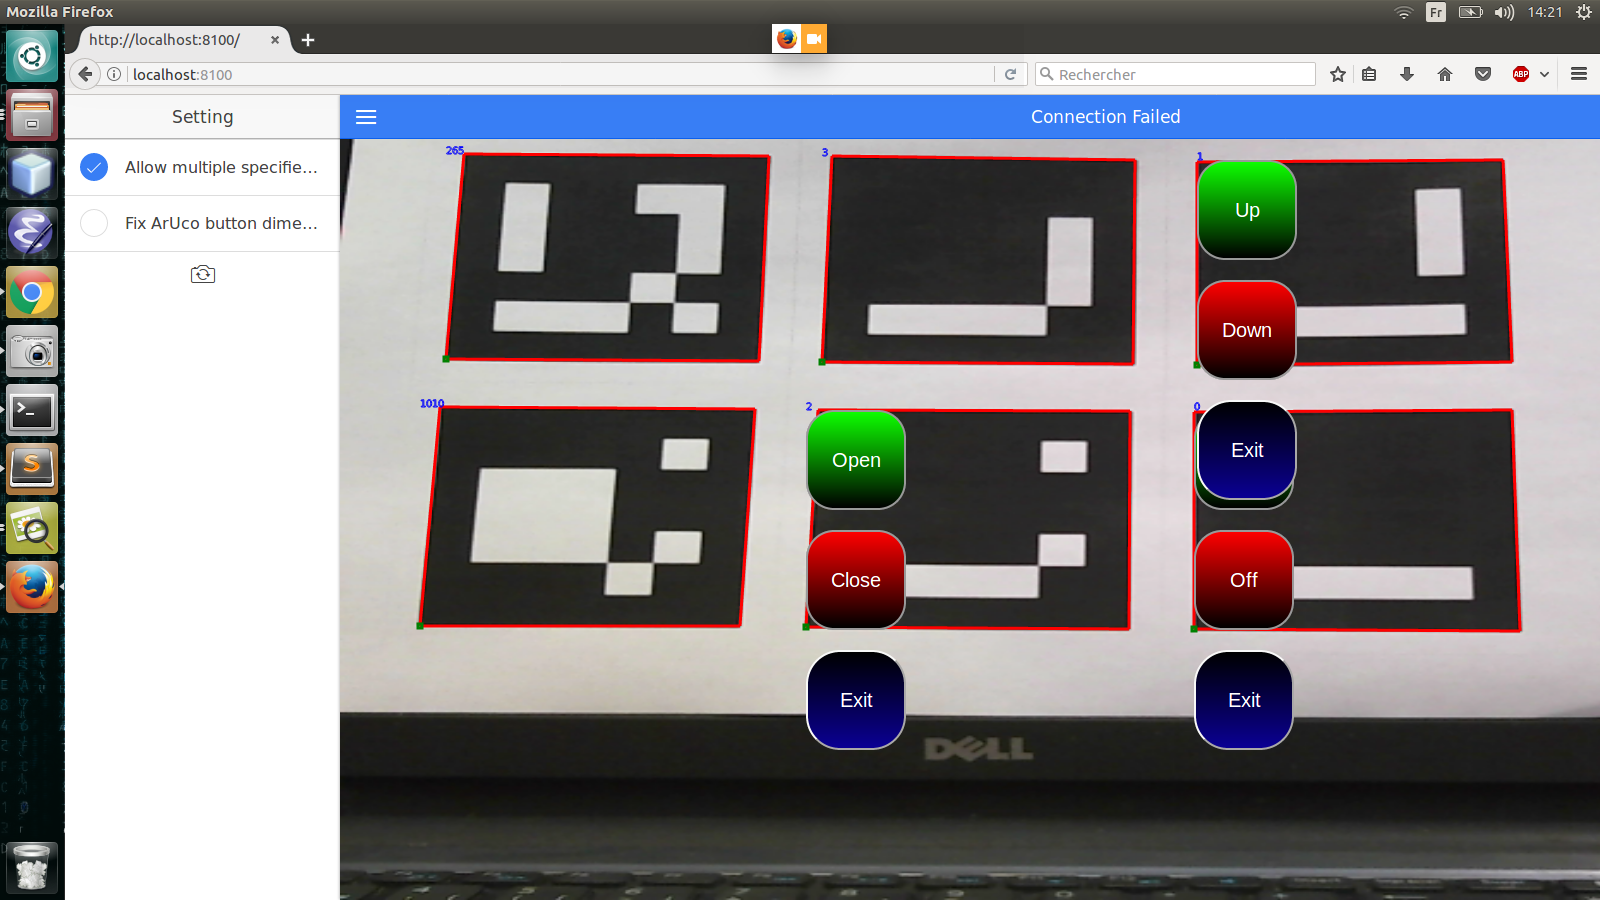
\includegraphics[width = 11cm,height=8cm]{2.png}
     \caption{Autoriser plusieurs interfaces.}
     \label{ihm2}

\end{figure}
\begin{figure}[H]
  \centering
    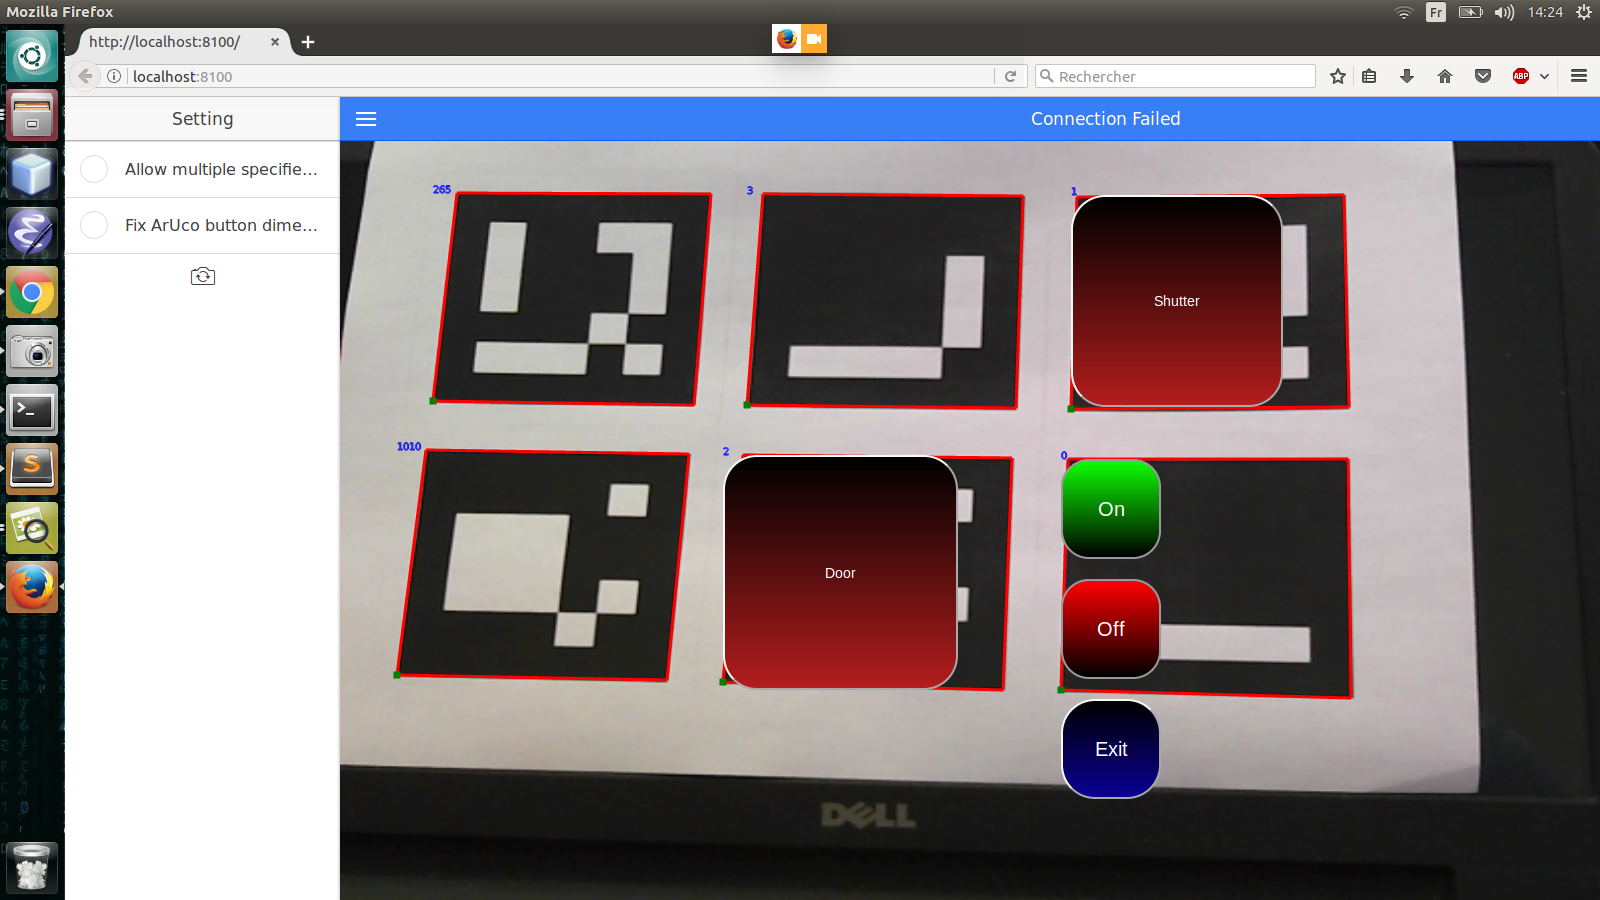
\includegraphics[width = 11cm,height=8cm]{4.png}
     \caption{Cas par défaut}
     \label{ihm2}
\end{figure}
\end{itemize}
\begin{itemize}
\item Redimensionner la taille des boutons, afin de rendre l'application plus accessible aux personnes à mobilité réduite.
\end{itemize}
\begin{figure}[H]
  \centering
    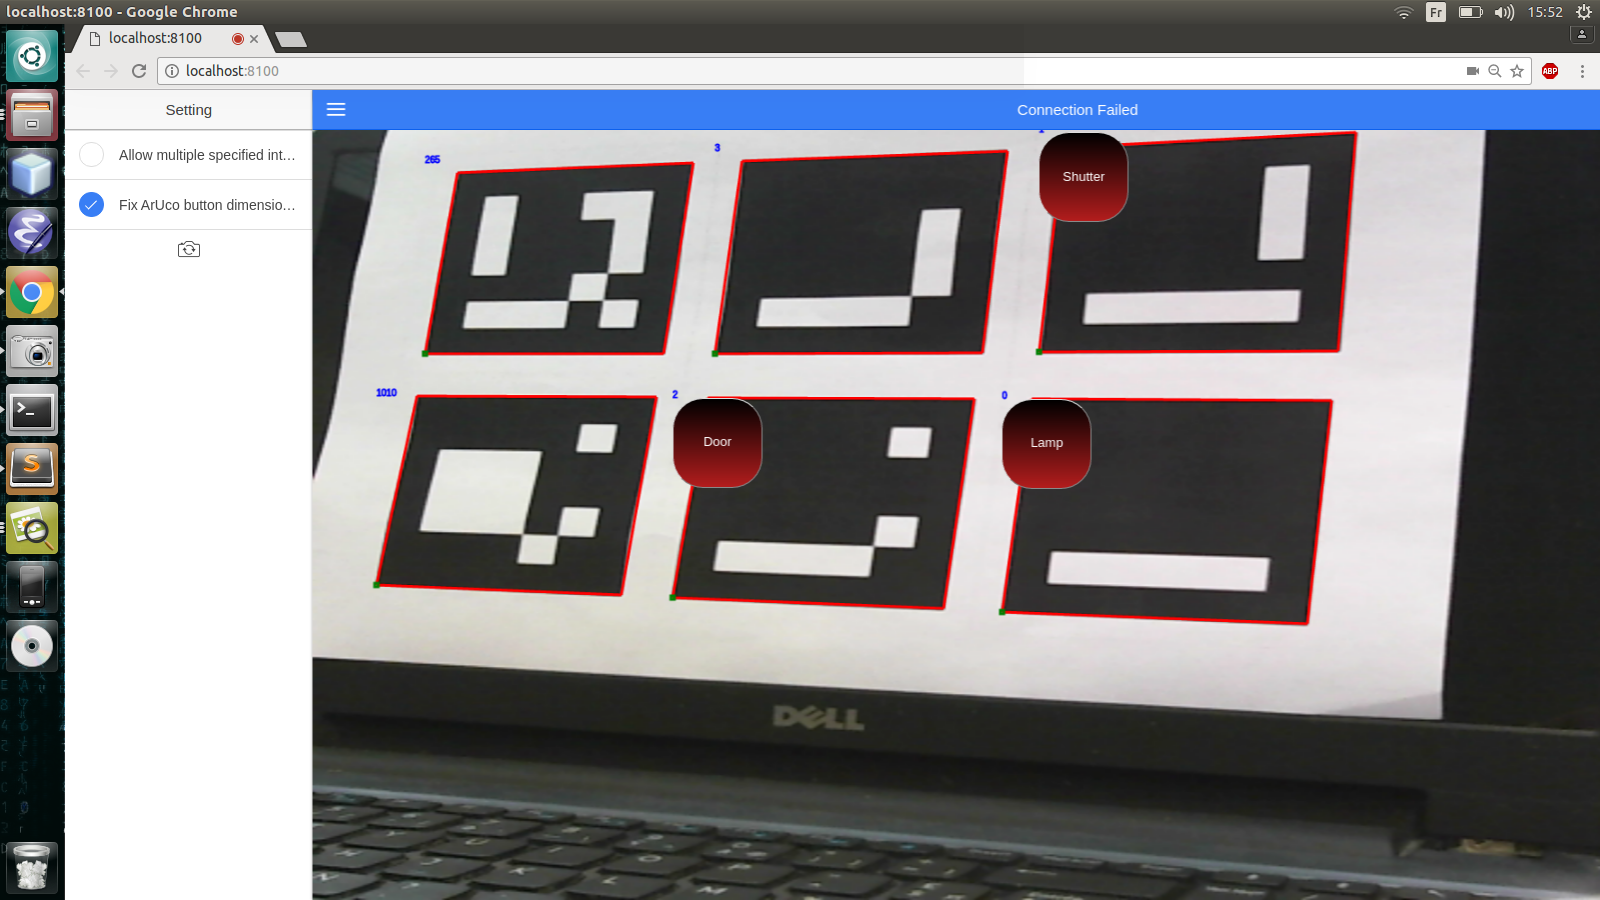
\includegraphics[width = 11cm,height=8cm]{6.png}
     \caption{Taille normale des boutons.}
     \label{ihm2}
\end{figure}

\begin{figure}[H]
  \centering
    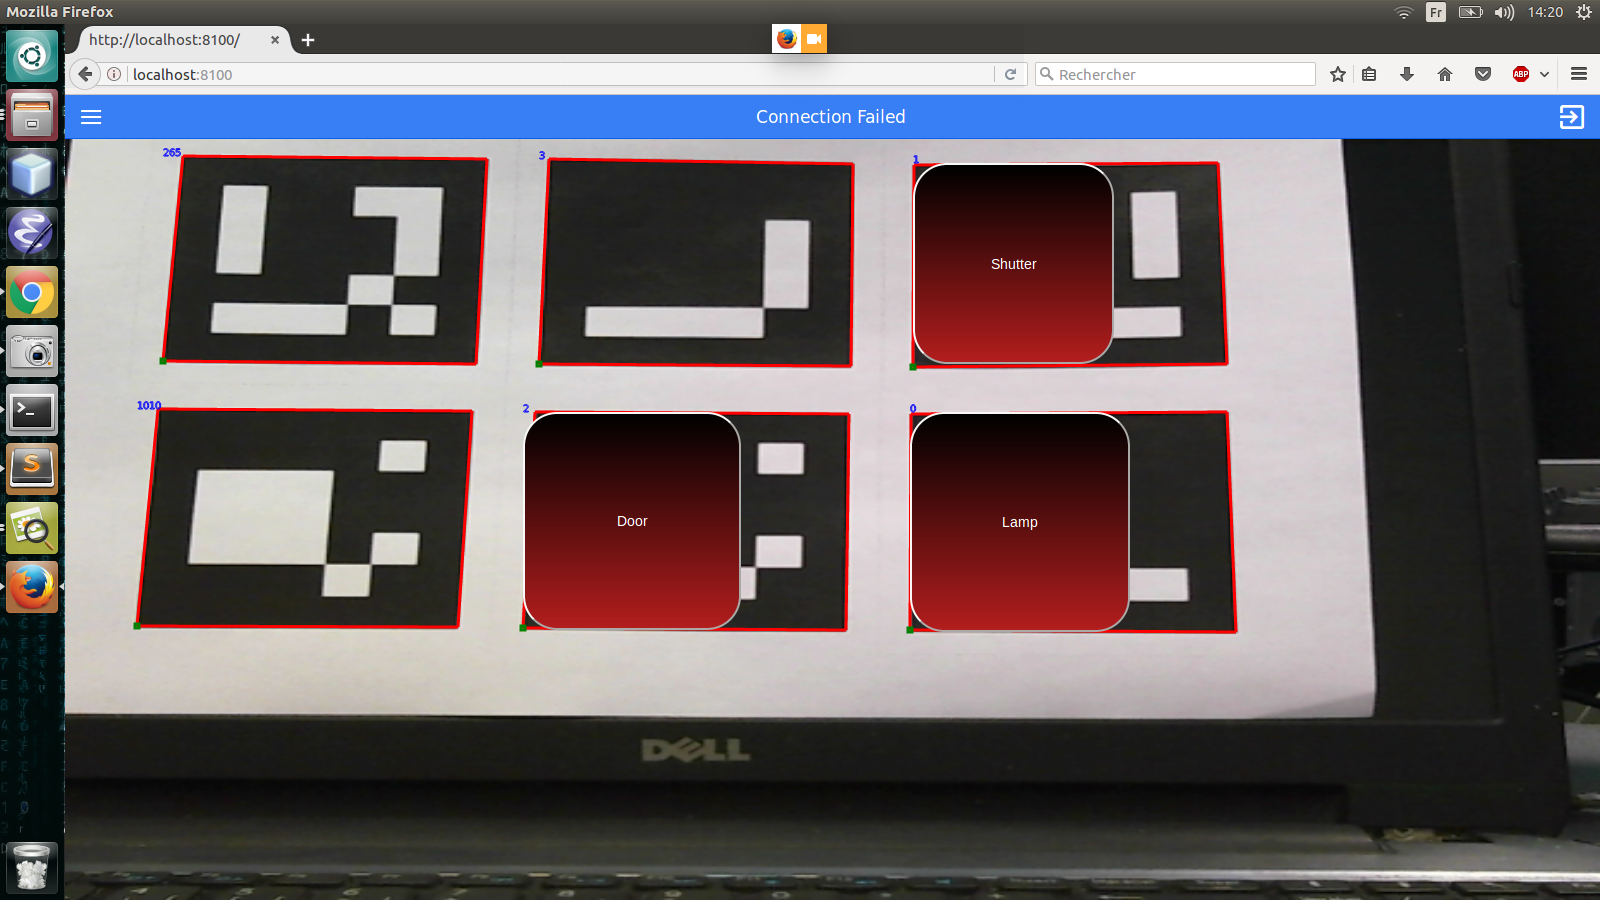
\includegraphics[width = 11cm,height=8cm]{3.png}
     \caption{Taille des boutons plus grande.}
     \label{ihm2}
\end{figure}
\begin{itemize}
\item Passer de la caméra arrière à la caméra frontale et inversement, en cliquant sur l’icône de la caméra.
\end{itemize}
\begin{figure}[H]
  \centering
    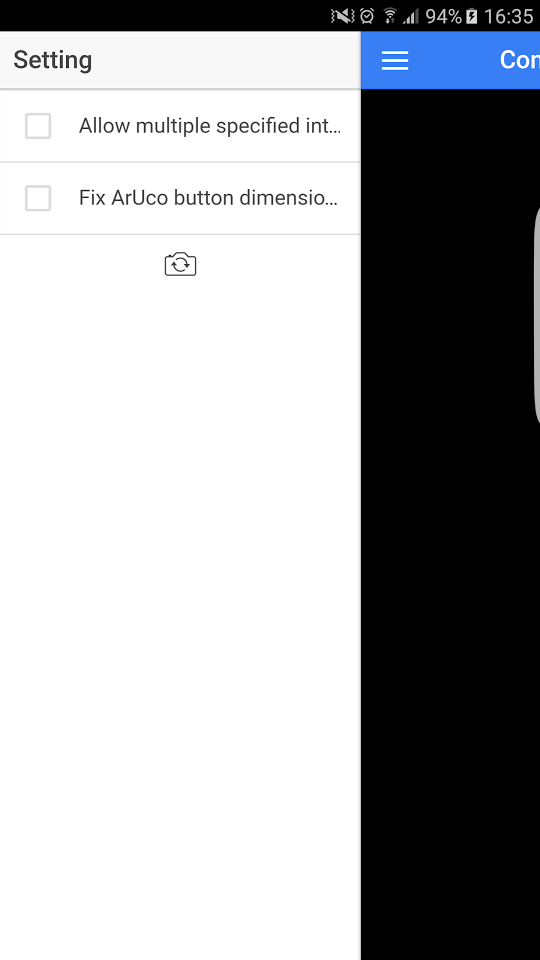
\includegraphics[width = 6cm,height=8cm]{7.png}
     \caption{changement de la caméra "frontale/arrière".}
\end{figure}
\end{itemize}

%Protocoles de communications et traitement de données
\subsection{Protocoles de communications et traitement de données}
Afin de faire communiquer notre application avec un Raspberry pi, nous aurons besoin d'un protocole de communication, nous avons opter pour le protocole MQTT(Cf.\cite{Ref21}).\par
En effet MQTT est un protocole essentiellement utiliser pour faire connecter des machines, dit protocole M2M (machine to machine), très utilisé dans le domaine de l'IoT (Cf.\cite{Ref27}), c'est un protocole léger fonctionnant selon un principe de publish/subscribe de messages, le rendant idéale à appliquer pour des solutions de domotiques. Étant un protocole relativement léger, consommant peu de ressources, communiquant via des paquets de taille minimale et efficace quand il s'agit de faire communiquer un appareil à un ou plusieurs autres, cela fait de lui un protocole idéale à intégrer dans des applications mobiles.\par 

\begin{figure}[H]
  \centering
    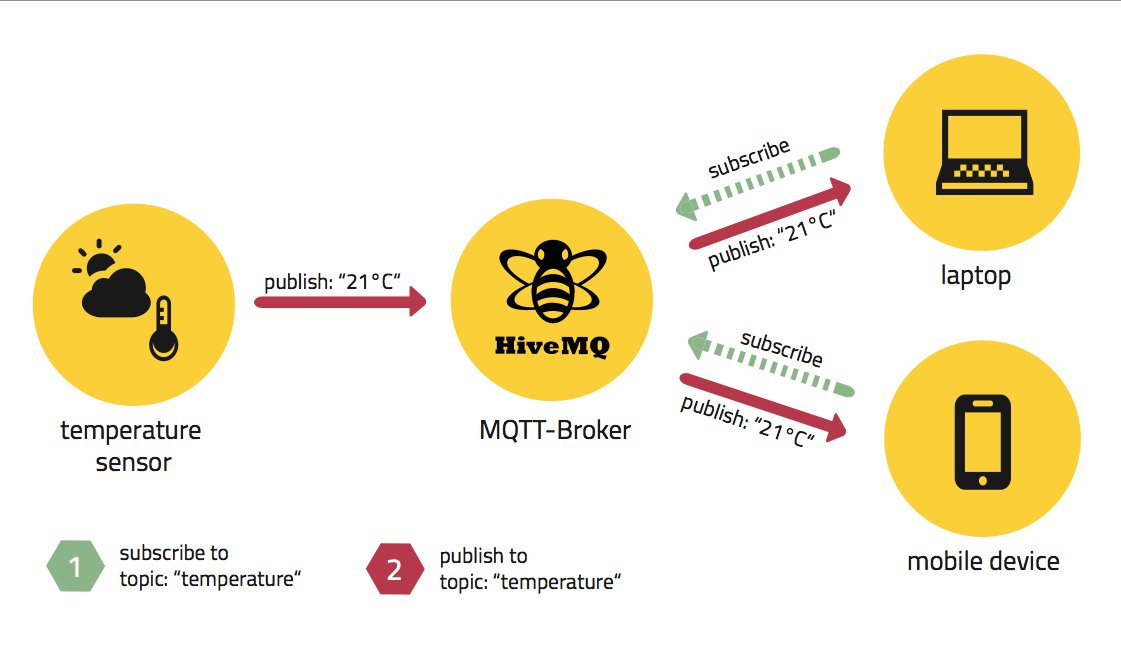
\includegraphics[width = 15cm,height=11cm]{mqtt_design.png}
     \caption{Principe de fonctionnement de MQTT}
     \href{url}{http://www.hivemq.com/blog/how-to-get-started-with-mqtt  }
     \label{prototype}
\end{figure}

	Cette figure (Cf.Figure ~\ref{prototype})	 illustre le principe de fonctionnement de MQTT. Tout d'abord, un appareil destiné à récupérer la température ambiante, publie son résultat dans un serveur Broker sous un topic nommé "temperature" dans ce cas la, des appareils à distances s'abonnent à ce topic "temperature" dans le serveur Broker à fin de récupérer l'information voulu (la température ambiante).\par
    
Dans notre cas nous avons utilisé le serveur Broker de test, disponible gratuitement en ligne et fournie par Mosquitto (Cf.\cite{Ref29}), c'est un serveur dédié à ce genre d'applications, dans la partie bilan et perspectives nous proposerons une manière d'implémenter son  propre serveur Broker Mosquitto et ce qu'il faut changer dans le code source de notre application afin de l’exploiter.\par
Passons maintenant aux choses concrètes, en se référant à notre diagramme de déploiement (partie Architecture logicielle), nous distinguons que la communication depuis l'application mobile vers le Raspberry PI se passe en deux étapes :

%Application mobile vers serveur Broker
\subsubsection{Application mobile vers serveur Broker}
C'est dans le fichier www/js/imageProcessing.js qu'est essentiellement implémenter cette partie.\par
Nous avons initié une connexion au serveur Broker sur le port 8080, le port pour les WebSockets fourni par le serveur Broker dédié de Mosquitto, puis nous nous sommes abonnés au topic nous permettant d'échanger des messages.\par

Puis dans le fichier /www/js/toServer.js nous avons déclaré les différentes méthodes nous permettant de publier des messages dans le serveur Broker afin de les échanger avec le Raspberry PI.\par
Cette figure (Cf.Figure ~\ref{the_server}) liste les différents ports de connexion fournis par le Broker dédié de Mousquitto.

\begin{figure}[ht]
\centering
	  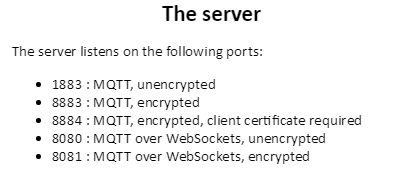
\includegraphics[width = 15cm,height=11cm]{mosquitto_test_ports.png}
     \caption{Ports de connexion fournies par le Broker dédié Mosquitto 
     \href{url}{http://test.mosquitto.org/}  }
	\label{the_server}
\end{figure}

%Serveur Broker vers Raspberry PI
\subsubsection{Serveur Broker vers Raspberry PI}
Cette partie a été développée en langage python, c'est plus tôt le Raspberry PI qui se connecte au serveur afin d'y récupérer les messages voulus.\par
A fin d'y procéder, nous avons utilisé les fonctionnalités fournies par la plate-forme de développement Paho, cette plate-forme implémente le protocole de communication MQTT.\par
Tout d'abord nous nous connectons au serveur Broker "test.mosquitto.org" sur le port numéro 1883, puis nous nous abonnons au topic en question via la fonctionnalité "publish", ce programme boucle à l'infini, et test à chaque fois le message récupéré du Broker, si par exemple le message est "ON", une condition est vérifiée et son contenue est exécuté, ce qui permet d'allumer une led. 
%Description de led
%Guide d'utilisation du matériel
\subsection{Guide d'utilisation du matériel}
Au cours de notre projet nous étions amenés à travailler sur du matériel, avant d'énumérer les tâches effectuées sur le matériel, le tableau ci-dessous englobe les composants électroniques nécessaires pour réaliser le prototype de notre application, ainsi que leur utilité.(L'ensemble du matériel est fourni par le client) : 
\par
\begin{table}[H]
\centering

\label{tableau3}
\begin{tabular}{|l|l|}
\hline
Materiel                      & Rôle                                                                \\ \hline
Chargeur  SAMSUNG(9V) & Alimenter le Raspberry                                              \\ \hline
Rasbperry pi-modèle b         & Communiquer avec notre application pour  allumer  une LED              \\ \hline
Carte SD (64GO)               & Espace de stockage de le Raspebrry                                  \\ \hline
Câble Ethernet (RJ45)         & Connecter le Raspeberry avec notre Pc                               \\ \hline
Breadboard                    & Dispositif pour réaliser le prototype de notre circuit électronique \\ \hline
Fils électriques              & Relier les composants de notre circuit                              \\ \hline
Résistance 280 ohms           & Protéger la LED de l'intensité du courant                           \\ \hline
Led rouge(DIODE)                     & Visualiser le fonctionnement de notre circuit.                      \\ \hline
\end{tabular}
\caption{Composants électroniques fournis}
\end{table}
\par
Nous allons maintenant détailler l'ensemble des étapes effectuées sur le matériel par ordre chronologique.\par 

%Installation du système d'exploitation sur le raspberry
\subparagraph{Installation du système d'exploitation sur le Raspberry :} 
Pour commencer la manipulation du Raspberry, il faut installer un système d'exploitation sur le Raspberry, cependant le Raspberry utilise une carte SD comme disque dur, pour cela il faut rendre la carte SD bootable avec le système d'exploitation. Pour notre cas on a opté pour le système d'exploitation "Raspbian'", ce dernier et un système basé sur Debian, il est optimisé pour fonctionner sur le Raspberry. En plus il est utilisé par une large communauté et il est supporté officiellement par le Raspberry.
L'installation s'avère simple il suffit de mettre l'image de Raspbien (294 MO) sur notre carte SD et suivre les instructions d'installation proposée graphiquement.\par

%Prendre le contrôle de la Raspberry:
\subparagraph {Prendre le contrôle du Raspberry:}
Il existe deux manières pour commander le Rasbperry : 
la première façon est de relier le Raspberry, avec du matériel (écran, clavier, USB) et l'utiliser comme un ordinateur fixe.
la deuxième méthode et celle qu'on a utilisée, connecter le Raspberry avec un ordinateur à l'aide d'un câble Ethernet, et établir une connexion ssh. Cette méthode reste plus pratique et rapide pour nos besoins.\par 

Pour établir une connexion ssh avec le Raspberry il faut d'abord configurer notre interface réseau, pour que notre ordinateur soit dans le même réseau que celui du Raspberry.
On précise ici que l'adresse Ip locale de notre Raspberry est \textbf{192.168.137.10} (définis lors de l'installation du 'Raspbian').\par 
\subparagraph{Connexion SSH sous Linux(Ubuntu):}On modifie le fichier \textbf{/etc/network/interfaces} pour attribuer une adresse IP statique (192.168.137.1), par exemple, pour valider les changements on exécute la commande :\textit{\textbf{service networking restart }}
.\par 

%Connexion SSH sous Windows:
\subparagraph{Connexion SSH sous Windows:} Dans le menu \textit{Network Connections}, on sélectionne l'interface réseaux graphiquement puis on autorise le partage de connexion, on renseigne l'adresse Ip de l'interface qui doit appartenir au même réseau que le Raspberry. 
On choisit un client, dans notre cas (Putty), on saisit l'adresse ip  et on se connecte.\par

%Connecter la raspberry à internet:
\subparagraph{Connecter le Raspberry à internet:} Connecter le Raspberry à internet demeure une obligation pour installer les bibliothèques nécessaires pour le fonctionnement de notre application(le protocole de communication exige la présence d'internet), pour connecter le Raspberry à internet on commence par scanner les réseaux Wi-Fi depuis notre Raspberry: la commande "\textbf{sudo iwlist wlan0 scan}" liste l'ensemble des réseaux Wi-Fi disponible, il renvoie un champ "\textbf{ESSID}'" qui sera utile plus tard. Ensuite il suffit d'ouvrir le fichier de configuration avec la commande : \textbf{sudo nano /etc/wpa-supplicant/wpa-supplicant.conf}, et ajouter les lignes suivantes :
%\begin{python}
%network={
  %  ssid="nom-resaux-wifi"
  %  psk="mot-de-passe-wifi"
%}
%\end{python}

\textbf{ssid} correspond au nom du réseaux wi-fi obtenu auparavant, psk est le mot de passe, enfin le Raspberry est connecter à internet.\par

%Allumer une LED depuis la raspberry:
\subparagraph{Allumer une LED depuis le Raspberry:} Allumer une LED est équivalent à un 'hello World' quand il s'agit de commencer avec le Raspberry, le but de cette partie sera de tester le bon fonctionnement des différents composants électroniques dont on dispose.
L’un des points les plus intéressants sur le Raspberry, est la partie GPIO : les ports GPIO (Général Purpose input/output) soit entrée/sortie, sont des ports qui sont très utilisés dans le monde des micro-contrôleurs, en particulier dans le domaine de l’électronique embarquée. Selon la configuration, ces ports peuvent fonctionner aussi bien en entrée qu’en sortie.
Les périphériques GPIO comportent un ensemble de ports d’entrée/sortie qui peuvent être configurés pour jouer soit le rôle d’une entrée, soit le rôle d'une sortie.(Cf.\cite{Ref18})
\par
Dans notre cas nous allons utiliser un port GPIO dédier pour clignoter une LED à partir d'un script python implémenter sur le Raspberry (Cf.Figure ~\ref{GPIO}).

\begin{figure}[ht]
\centering
	  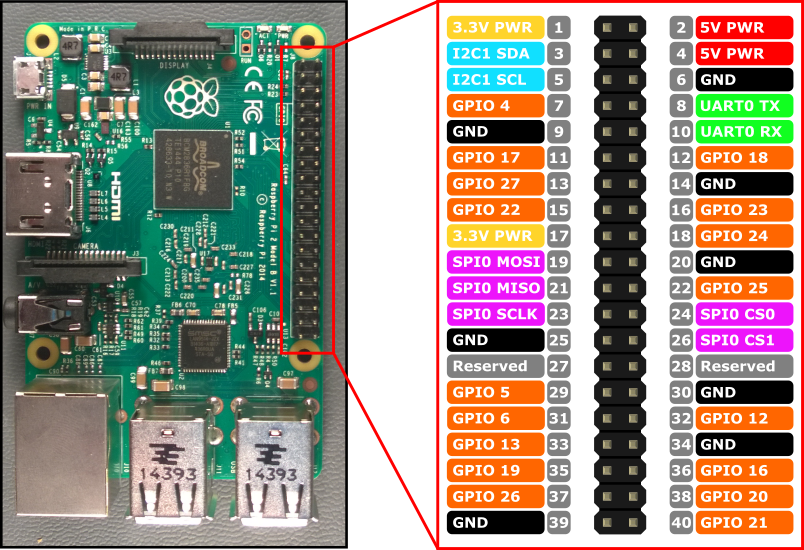
\includegraphics[width = 15cm,height=11cm]{pinout.png}
     \caption{Ports GPIO du Raspberry pi 3 model B 
     \href{url}{https://developer.microsoft.com/en-us/windows/iot/docs/pinmappingsrpi}  }
	\label{GPIO}
\end{figure}

Maintenant on va réaliser le montage du circuit électronique, pour cela on va brancher une LED et une résistance sur la breadboard, on relie les ports GPIO de la Raspberry avec le circuit implémenté sur la breadboard à l'aide des fils électriques, le circuit obtenu correspond à la figure suivante : \par
\begin{figure}[H]
  \centering
    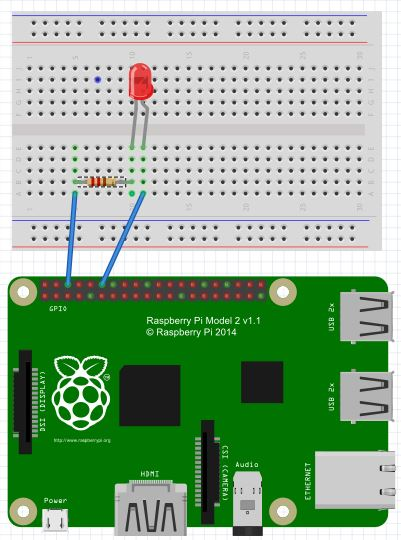
\includegraphics[width = 15cm,height=15cm]{led.png}
     \caption{Circuit électronique permettant d'allumer une LED avec un Raspberry
     \href{url}{http://www.geekland-leblog.fr/faire-clignote-une-led-en-python/}  }
\end{figure}
Après le branchement du matériel, on peut allumer la LED, pour cela il faut ajouter un script python comme cité auparavant. on va utiliser une bibliothèque python intitulée "\textbf{RPI.GPIO}", cette bibliothèque permet de contrôler les ports GPIO de le Raspberry, en associant un numéro de port GPIO à un état logique.
on commence par installer la bibliothèque : 
\begin{lstlisting}
sudo apt-get install python-dev python-rpi.gpio
\end{lstlisting}
on crée un fichier \textbf{led-test.py}, et on implémente le script python suivant :

Enfin on exécute \textit{led-test} : \newpage

\begin{python}
import RPi.GPIO as GPIO  # Framework to use GPIO

GPIO.setmode(GPIO.BOARD) # set pin configuration mode to Raspberry
GPIO.setup(7,GPIO.OUT)  # use pin number 18

 GPIO.output(7,GPIO.HIGH) # turn on the led
 GPIO.output(7,GPIO.LOW) #turn off the led 
\end{python}
\begin{figure}[ht]
  \centering
    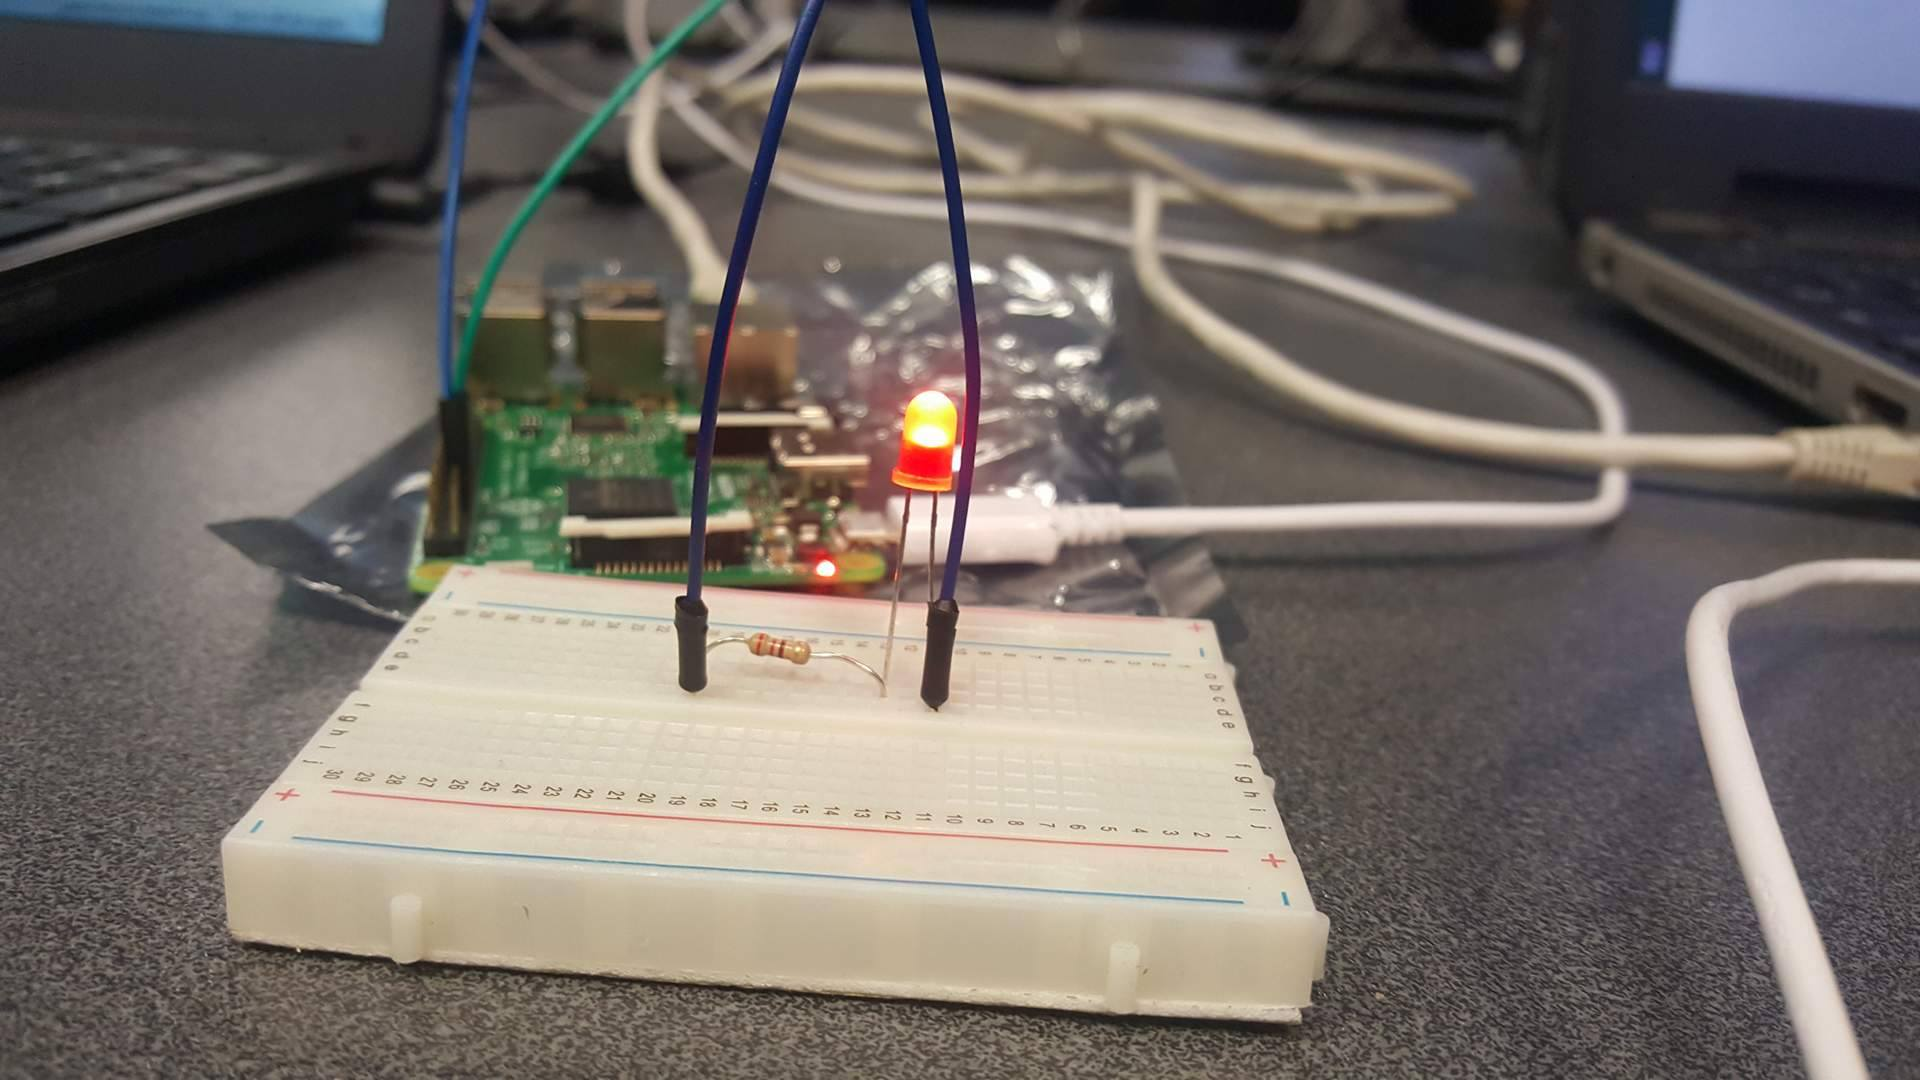
\includegraphics[width = 15cm,height=11cm]{led2.png}
     \caption{Notre propre LED est maintenant allumée ! 
      }
\end{figure}

%Tests
\section{Tests}
Afin de bien vérifier la validité de notre implémentation du coté matériels, on a implémenté des programmes de test.\par

\subsection{Test de fonctionnement des ports GPIO du Raspberry PI}
Le premier test consiste en, la vérification du bon état de marche de tous les ports GPIO du Raspberry PI.\par
Le test est implémenté dans le fichier python "GPIO\_test.py", tout d'abord, on introduit le numéro de port du GPIO sous forme d'entier. 

%Résultats
\subsubsection{Résultats}
Si le numéro de port entré est valide, on fait clignoter la LED branchée dans ce GPIO avec un intervalle de 0.5 secondes, si le numéro de port n'est pas valide, une exception est levée, indiquant l'erreur en question, sinon on indique que le port n'est pas fonctionnel.\par
Ce test pourra être implémenté dans l'application afin de diagnostiquer le bon fonctionnement des ports GPIO du Raspberry PI à distance, l'utilisateur pourra connaître les ports fonctionnels et non fonctionnels de son Raspberry PI après que ce diagnostic s'affiche sur l'interface correspondante. 

\subsection{Test de vérification du bon envoie d'un message via MQTT}
Pour cette partie, nous avons implémenté deux programmes en python, un premier, intitulé "test\_subscriber.py", qui se charge de s'abonner à un topic dans le serveur broker gratuit "test.mosquitto.org" en initiant une connexion via le numéro de port "1883", en s'abonnant, le programme se met en mode écoute, et affiche n'importe quel message publier dans le même topic.\par
Le deuxième programme, intitulé "test\_publisher.py", initie la même connexion que le programme précédent puis publie un message de test dans le même topic.
\subsubsection{Résultats}
\begin{figure}[H]
  \centering
    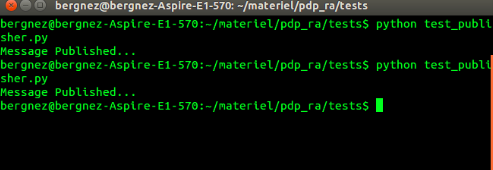
\includegraphics[width = 15cm,height=8cm]{19publish.png}
     \caption{Le publisher publie le message }
\end{figure}
\begin{figure}[H]
  \centering
    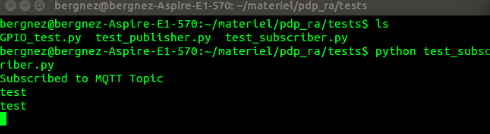
\includegraphics[width = 15cm,height=8cm]{19subscr.png}
     \caption{Le subscriber a bien reçus le message du publisher 
      }
\end{figure}
Tout d'abord, ce test démontre bien que le serveur "Broker" utilisé par l'application afin d'échanger des messages avec le Raspberry PI est fonctionnel.\par
Ce test pourra être exploité afin de vérifier d'autres "Broker" existant, ainsi si le "Broker" que nous avons utilisé tombe en panne, l'utilisateur pourra tester d'éventuels "Broker" et les utiliser si ils sont opérationnels, il pourra aussi tester le bon état de marche de son propre "Broker".

\subsection{Tests de robustesse}
Afin de tester la robustesse de notre application, nous avons utilisé certains outils spécifiques :
\subsubsection{Analyse des ressources utilisées par notre application via GameBench}
Nous avons tout d'abord analysé notre application sur une durée de 15 minutes via GameBench, ce test nous donnes des informations sur les ressources utilisées par notre application, 41 \% du CPU (processeur), 8 \% pour le GPU (processeur graphique) et 393 MO pour la mémoire vive sont utilisés par notre application. Sans oublier le fait qu'elle génère 9 images par seconde en moyenne.\par  
\begin{figure}[ht]
  \centering
    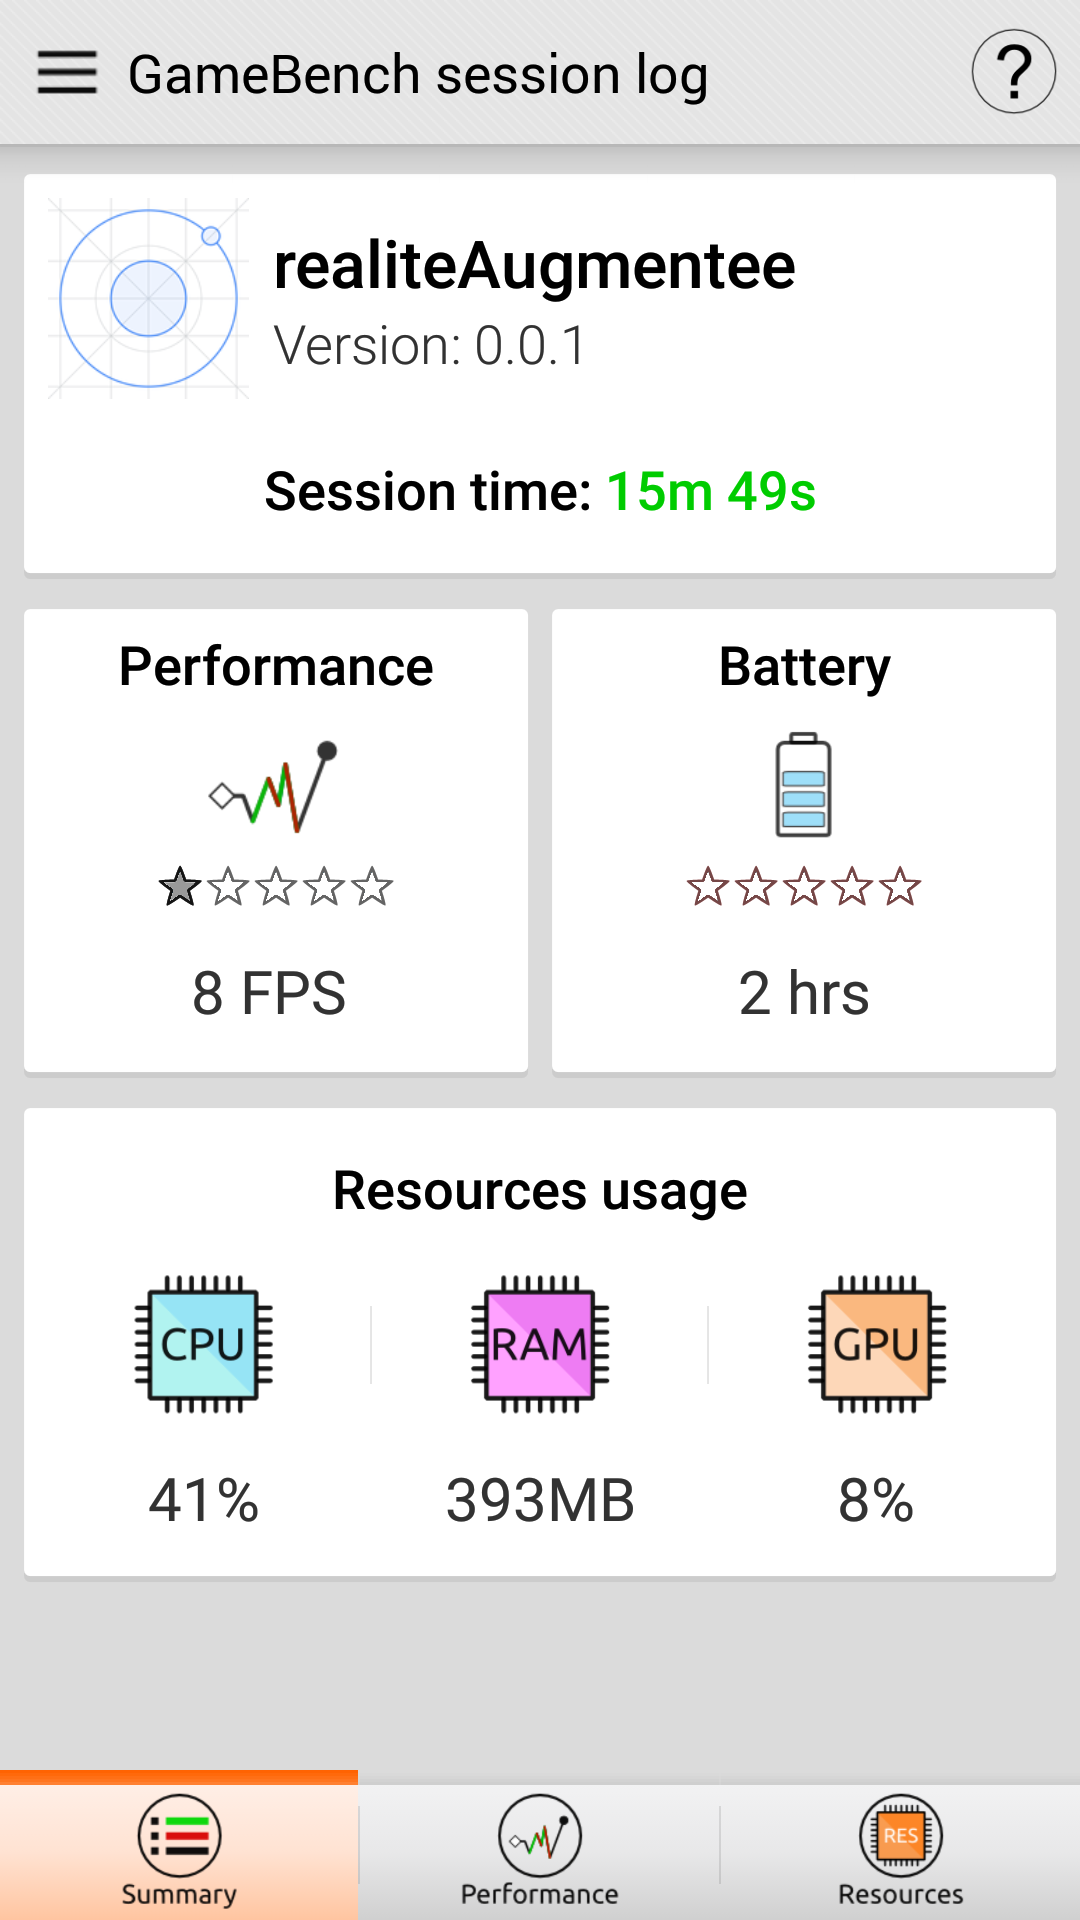
\includegraphics[width = 7cm,height=11cm]{test_gamebench_1.png}
     \caption{Ressources utilisées par l'appareil 
      }
      \label{premi_graphe}
\end{figure}
Le premier graphe(Cf. Figure ~\ref{graphe})  nous montre que sur une durée de 15 minutes, l'application consomme entre 10 \% et 60 \% du CPU.\par 
Le deuxième graphe (Cf. Figure ~\ref{graphe}) nous donne des informations sur les ressources GPU consommées, on constate que le CPU n'est trop monopolisé par notre application, de même pour le GPU, ce qui est positif pour nous.\par 
\begin{figure}[H]
  \centering
    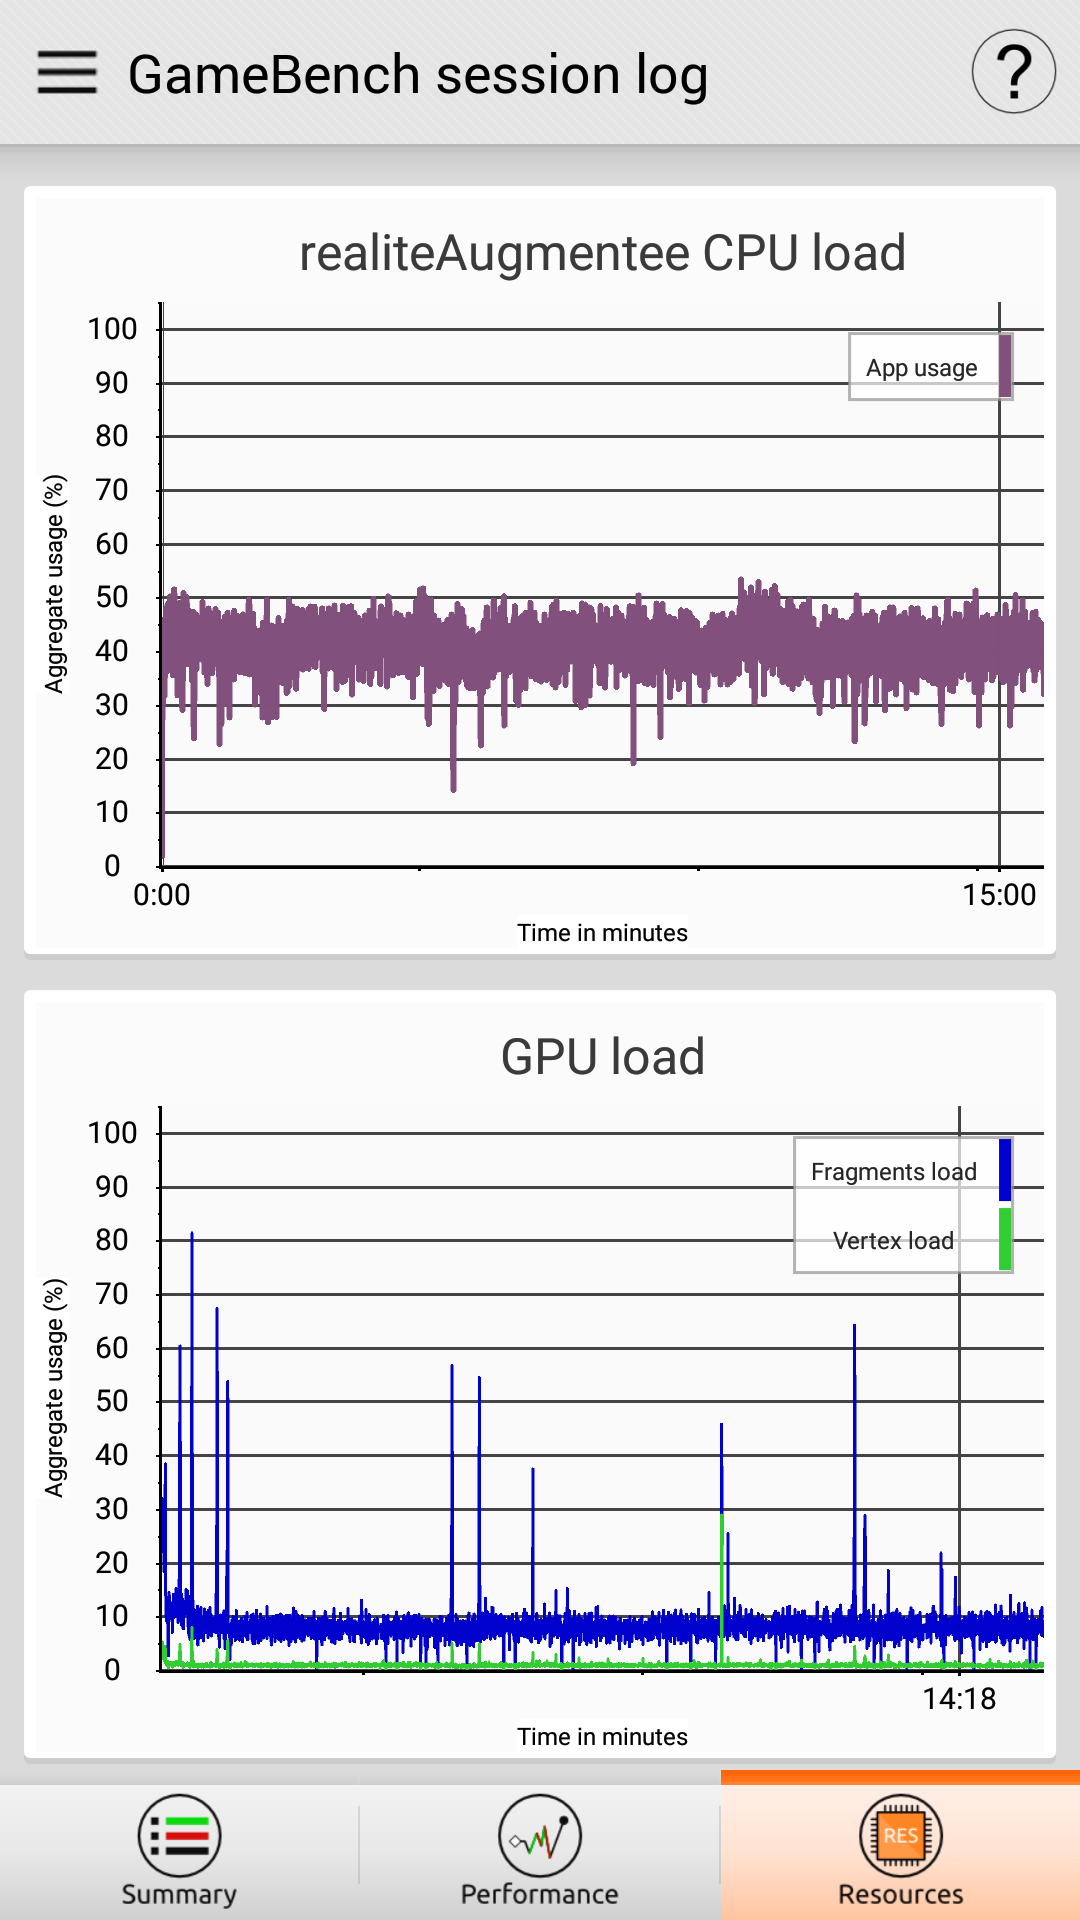
\includegraphics[width = 7cm,height=9cm]{test_gamebench_2.png}
     \caption{Graphe détaillant le pourcentage d'utilisation du CPU et du GPU }
     \label{graphe}
\end{figure}
La dernière figure (Cf. Figure ~\ref{ips}) nous montre que l'application génère entre 5 et 16 images par seconde sur une durée d'exécution de 15 minutes.\par
\begin{figure}[H]
  \centering
    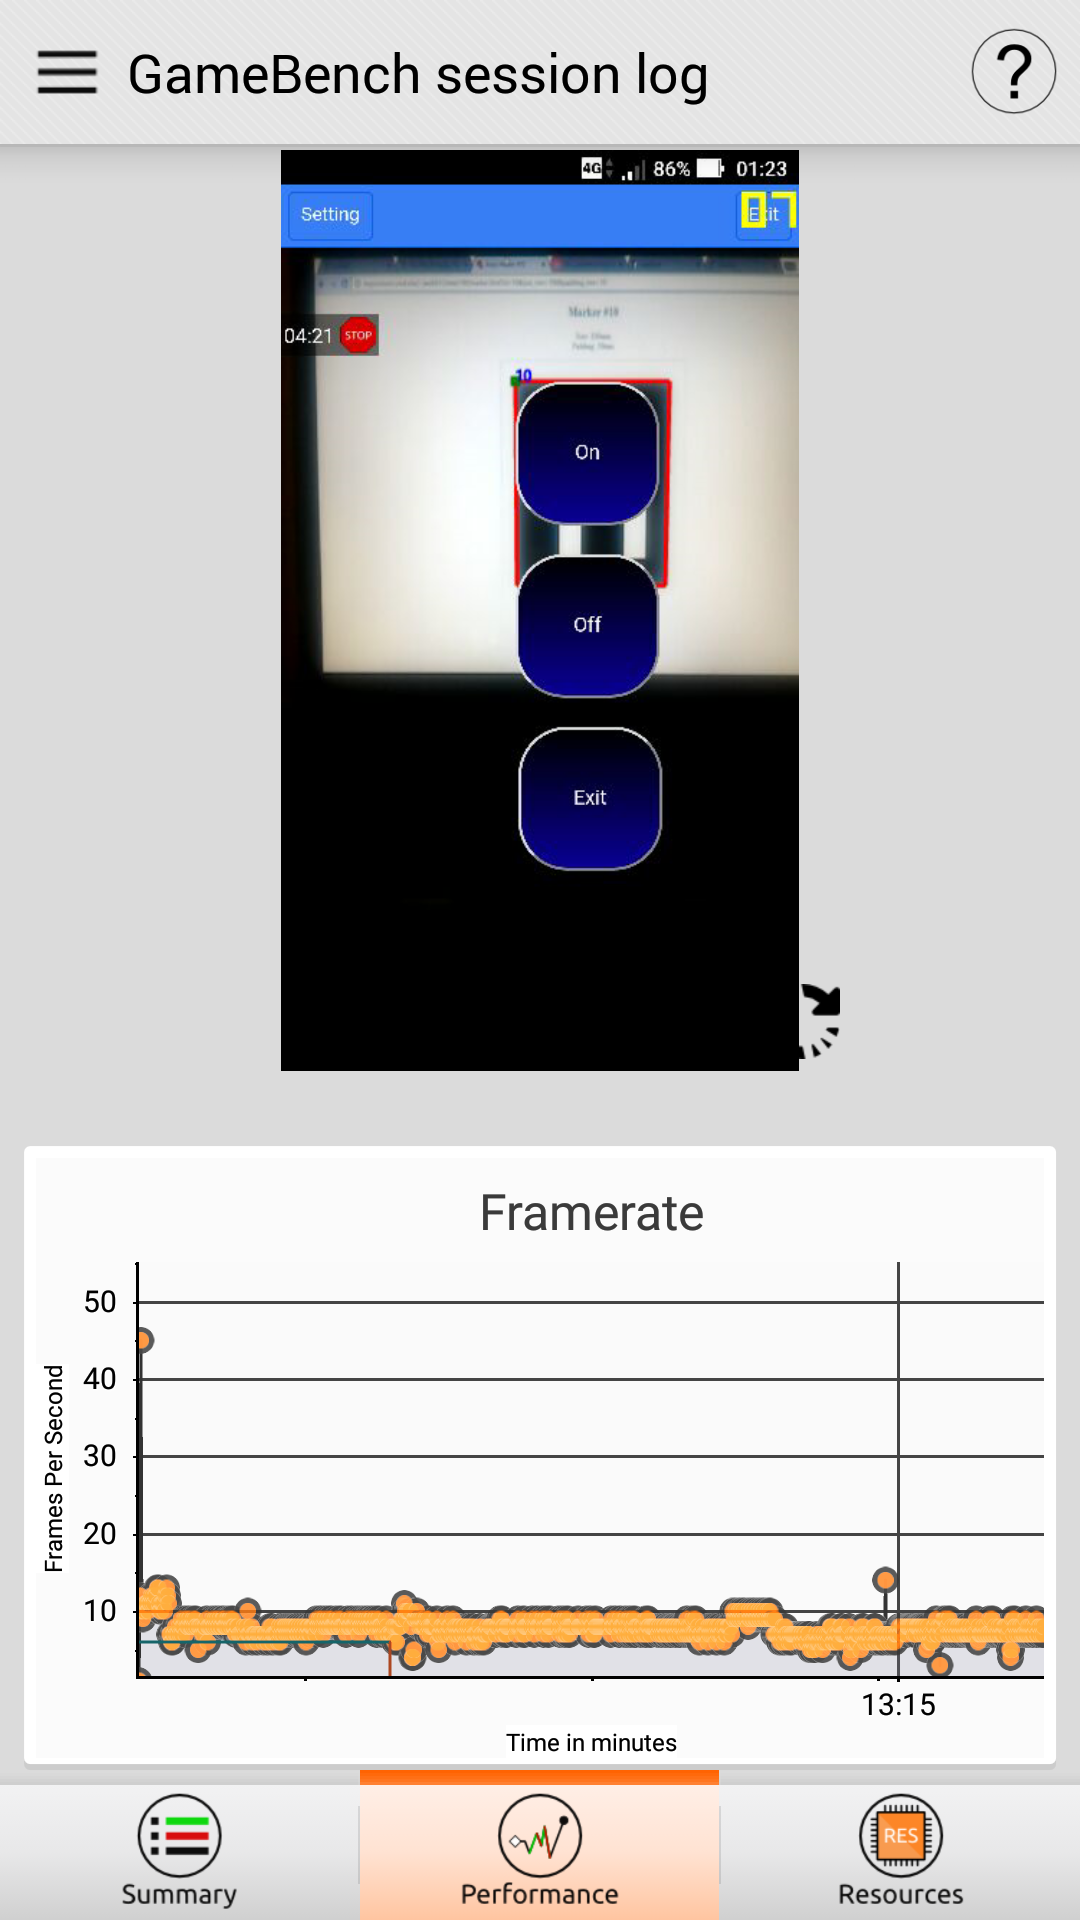
\includegraphics[width = 7cm,height=9cm]{test_gamebench_3.png}
     \caption{Taux d'ips généré par notre application 
      }
      \label{ips}
\end{figure}
Tous ces tests ont été effectuer sur un Smartphone de type Asus Zenforce 2~\ref{table1}.\par
\subsubsection*{Résultats :}
Pendant ce test, d'une durée de 15 minutes, nous avons exposé notre application à plusieurs cas extrêmes, en occurrence la reconnaissance de quatre marqueurs "ArUco" à la fois ainsi que la navigation dans leurs interfaces simultanément.\par
Les ressources utilisées par le CPU et le GPU, tout au long du test, ne présentent pas un écart important, ce qui prouve que l'utilisation intensive de l'application ne provoque pas une consommation gourmande au niveau du CPU et du GPU, par contre, le taux d'images par seconde n'est pas constant tout au long du test, il varie entre 45 et 4 images par seconde. Le taux d'images par seconde peut être amélioré en optimisant les calculs effectués par la bibliothèque JS-ArUco.  
\subsection{Tests de réactivité}
Afin de tester la réactivité de notre application, on a calculé directement le temps pris par l'application pour reconnaître un marqueur ArUco.\par
On a fait de même pour mesurer le temps de transmissions d'un message entre l'application et le Raspberry PI.
\begin{figure}[H]
  \centering
    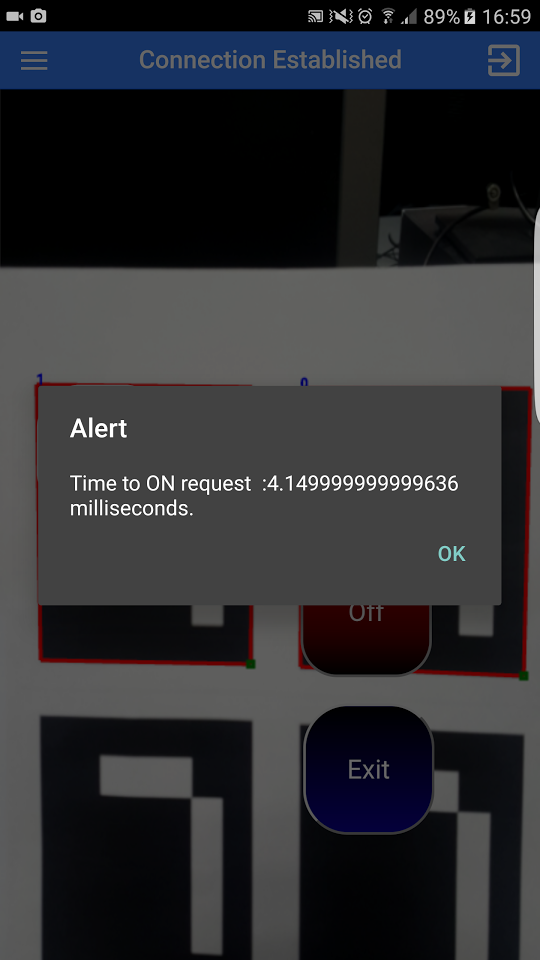
\includegraphics[width = 7cm,height=8cm]{17.png}
     \caption{Temps d’échange avec le serveur.}
     \label{fig29}
\end{figure}

\begin{figure}[H]
  \centering
    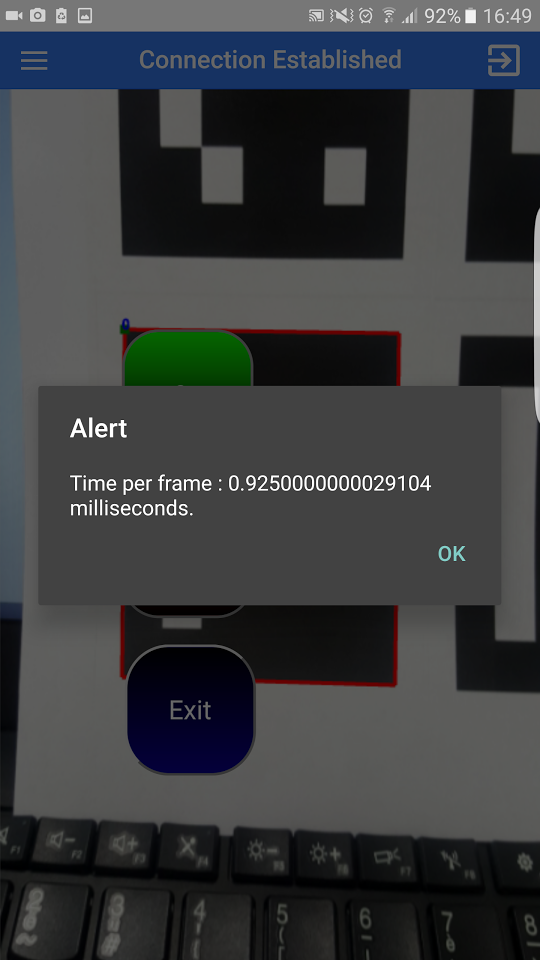
\includegraphics[width = 7cm,height=8cm]{12.png}
     \caption{Temps de reconnaissance du marqueur Aruco.}
     \label{fig28}
\end{figure}
\subsubsection{Résultats :}
Les temps respectent les normes qu'on a définies dans les besoins non fonctionnels, ainsi on assure la réactivité de notre application.
% * <chaouchi.aghiles@outlook.com> 2017-04-04T11:46:00.144Z:
%
% ^.
%Bilan et perspectives
\section{Bilan et perspectives}

Avant de commencer à développer l'application, nous avons tout d'abord rédigé un cahier de charges qui a été itéré plusieurs fois, nous nous sommes tout d'abord occupé de la partie besoins fonctionnels, nous l'avons partitionné en quatre parties qui sont respectivement ; "Traitement d'images", "Interface homme-machine", "Accessibilité pour les personnes à mobilité réduite" et "Protocoles de communications et traitement de données", nous avons consulté nos clients régulièrement afin de bien comprendre leurs besoins, puis nous sommes passé aux besoins non fonctionnels qui demeurent une partie très importante du cahier de charges, nous avons surtout bien discuté avec nos clients sur les contraintes de développement qui nous sont imposées, notamment le fait que les plate-formes de développement utilisées doivent être sous licence GPL ou LGPL, que nous avons respecté.\par

Ensuite nous sommes passés à la partie cas d'utilisation, nous avons bien représenté les scénarios proposés par nos clients. \par

Une fois que de bonnes bases ont été construites, nous sommes passés à la partie développement et construction de l'architecture du logiciel. \par

Le développement de l'application s'est passé en quatre étapes qui sont les suivantes : \par

\subparagraph{Traitement d'images :}
Nous avons pu récupérer le flux vidéo de la caméra d'un smartphone, ceci étant une partie indispensable pour la suite, ensuite nous avons exploité les travaux de Juan Mellado comme cité dans la partie "Code - Traitement d'image", ses travaux nous ont permis de reconnaitre des marqueurs ArUco en temps réel, de les encadrer avec un rectangle rouge, et de récupérer leurs contenues.\par

\subparagraph{Création de l'interface graphique :}

Une fois la partie traitement d'images terminée, nous avons commencé à implémenter l'interface graphique, qui permet à l'utilisateur d'interagir avec son environnement et de pouvoir donc piloter des appareils à distance. Comme détaillé dans la partie "Code - Interface homme-machine", nous avons développé notre application avec la plate-forme de développement Ionic, nous nous sommes donc servis des composants graphiques fournis par ce dernier afin d'implémenter notre interface graphique, Si un marqueur ArUco est reconnu par notre application, on affiche un bouton sur le marqueur, jusqu'à arriver à une interface spécifique, qui selon le choix de l'utilisateur, récupère un traitement à effectuer sur un appareil distant.\par

De plus nous nous sommes préoccupés de l'aspect accessibilité pour les personnes à mobilité réduite, afin de rendre notre application plus accessible à ce genre de personne.\par

\subparagraph{Connexion de l'application avec le Raspberry PI :}

Nous nous sommes servis de la plate-forme de développement Paho, qui implémente le protocole de communication MQTT, et à la fin, nous avons donc réussi à faire communiquer l'application avec le Raspberry PI.\par

\subparagraph{Mise en place d'un circuit électronique :}

Nous avons mis en place un circuit électronique basique, comportant une simple LED, et nous avons réussi à l'allumer depuis l'application, nous avons simulé le fonctionnement de l'application, en identifiant la LED par un marqueur ArUco, puis nous nous sommes servis de l'application pour identifier ce marqueur, une fois qu'une interface spécifique s'est affichée, nous nous sommes servi de cette dernière pour piloter la LED, c'est-à-dire l'allumer et l'éteindre.\par

Ceci démontre bien le fonctionnement de notre application et la réalisation de notre projet, en effet des modifications devront être apportées dans le côté matériel afin de pouvoir manipuler de vrais appareils (des lampes, des téléviseurs ...)\par

Nous avons donc réussi à remplir les tâches qui nous ont été confiées.\par

A la fin, nous avons fait subir un test de robustesse à notre application, afin de connaître les ressources utilisées par notre application, notre application ne consomme pas trop de mémoire vive, elle ne monopolise pas trop le CPU ni le GPU, mais elle ne génère qu'un taux de 9 images par seconde en moyenne sur l'appareil avec lequel on l'a testé, ce qui peut être amplement amélioré.\par


Le sujet qu'on a choisi dans le cadre du projet de programmation, nous a permis d'élargir nos connaissances dans différents domaines, il nous a surtout permis de nous initier au domaine du génie logiciel, à travers la rédaction d'un cahier de charges, la répartition des tâches et le travail de groupe, la mise en place de tests, le respect des délais imposés, les rendez-vous avec les clients, au-delà des aspects techniques, cela nous a permis de nous sensibiliser aux besoins des personnes à mobilité réduite en matière de logiciels et applications afin de contribuer à leur confort.\par

\subsection*{Problèmes rencontrés :}

Nous avons rencontré des difficultés au début, car nous n'avons jamais travaillé avec des outils tels que Ionic, de plus, c'était la première fois qu'on devait travailler avec des composants électroniques tels que le Raspberry PI, nous devions donc pallier ces problèmes en se plongeant dans diverses documentations. \par

Nous allons maintenant présenté nos perspectives afin qui serviront à améliore notre projet.\par

\subsection*{Perspectives :}

\subparagraph{Mettre en place les cas d'utilisations}
Dans un premier temps, nous avons réalisé un prototype qui permet d'allumer une LED, mais notre projet ne se limite pas qu'a ça, on voudrait dans un deuxième temps, implémenter tous les cas d'utilisation que nous avons proposé, c'est-à-dire, manipuler les volets d'une fenêtre, commander une télévision... La mise en place se fera en intervenant qu'au niveau matériel  afin de pouvoir manipuler ces appareils, vu que la partie application et serveur est achevée.

\subparagraph{Compatibilité :} L'application sera compatible avec les plate-formes : Android 5.0, Ios 8 et Windows Phone 8.1.(versions minimums supportées par Cordova)\par

\subparagraph{Installer son propre Broker Mosquitto :}
Pour le déploiement de notre application, nous avons utilisé un serveur Broker fourni par Mosquitto comme décrit dans la partie "réalisation", mais pour des raisons de sécurité et d'autonomie on peut déployer son propre serveur Broker sur internet ou en local, un bon tutoriel en anglais, proposé par DigitalOcean peut être trouvé sur ce lien (Cf.\cite{Ref31}).\par

\subparagraph{Ajouter des sessions d'utilisateurs :}
Dans notre diagramme de classe, nous avons présenté une classe "Session" ainsi qu'une classe "Storage" que nous n'avons pas pu intégrer à temps, la classe "Session" permet à un utilisateur de s’authentifier avant d'utiliser l'application, ce qui permet d'assigner à l'utilisateur des privilèges spécifiques sur des appareils, et donc protéger l'accès à certains appareils, nous proposons en tant que perspective de synchroniser l'application avec un serveur, c'est-à-dire, dans un premier temps, l'utilisateur clique sur un bouton, ce n'est qu'après qu'une première requête soit envoyée vers ce serveur afin de vérifier si l'utilisateur en question détient les droits nécessaires pour pouvoir manipuler cet appareil, qu'une interface spécifique s'affiche ou pas sur le bouton.\par
C'est dans la classe "Storage" que les identifiants des utilisateurs sont assignés aux identifiants des marqueurs, le serveur y puisera pour connaître qui a droit de manipuler quoi.
\subparagraph{Amélioration de l'interface graphique}
Pour l'instant on se limite à afficher des boutons simples sur l'interface graphique afin de manipuler les appareils, ceci ayant pour but de simplifier l'interaction avec l'application pour les personnes à mobilité réduite.\par
Nous proposons de mieux introduire l'aspect de la réalité augmentée, en remplaçant les boutons par une interface en deux dimensions prenant la forme concrète de l'appareil à manipuler.\par
Un exemple concret serait, une interface en forme de lampe en 2 dimensions s'affichant sur le flux vidéo d'un smartphone quand un utilisateur essaye de manipuler une lampe

\newpage

%Annexes
\section{Annexes}
\subsection{Cas d'utilisations}
\subsubsection{Cas d'une fenêtre}
\begin{itemize} 
  \item L'utilisateur pointe sa tablette sur un marqueur ArUco.
  \item Le système détecte le code ArUco et y affiche un bouton d'activation. 
  \item L'utilisateur sélectionne le code ArUco en cliquant sur le bouton spécifique.
  \item Le système affiche une interface spécifique à la fenêtre.
  \item L'utilisateur demande de descendre ou faire monter les volets via l'application.
  \item Le système envoie la requête au serveur web.
  \item Le serveur traite la requête et l'envoie au Raspberry PI.
  \item Le Raspberry PI exécute l'ordre et fait donc monter ou descendre les volets.
\end{itemize}
\newpage
\begin{figure}[h!]
  \centering
  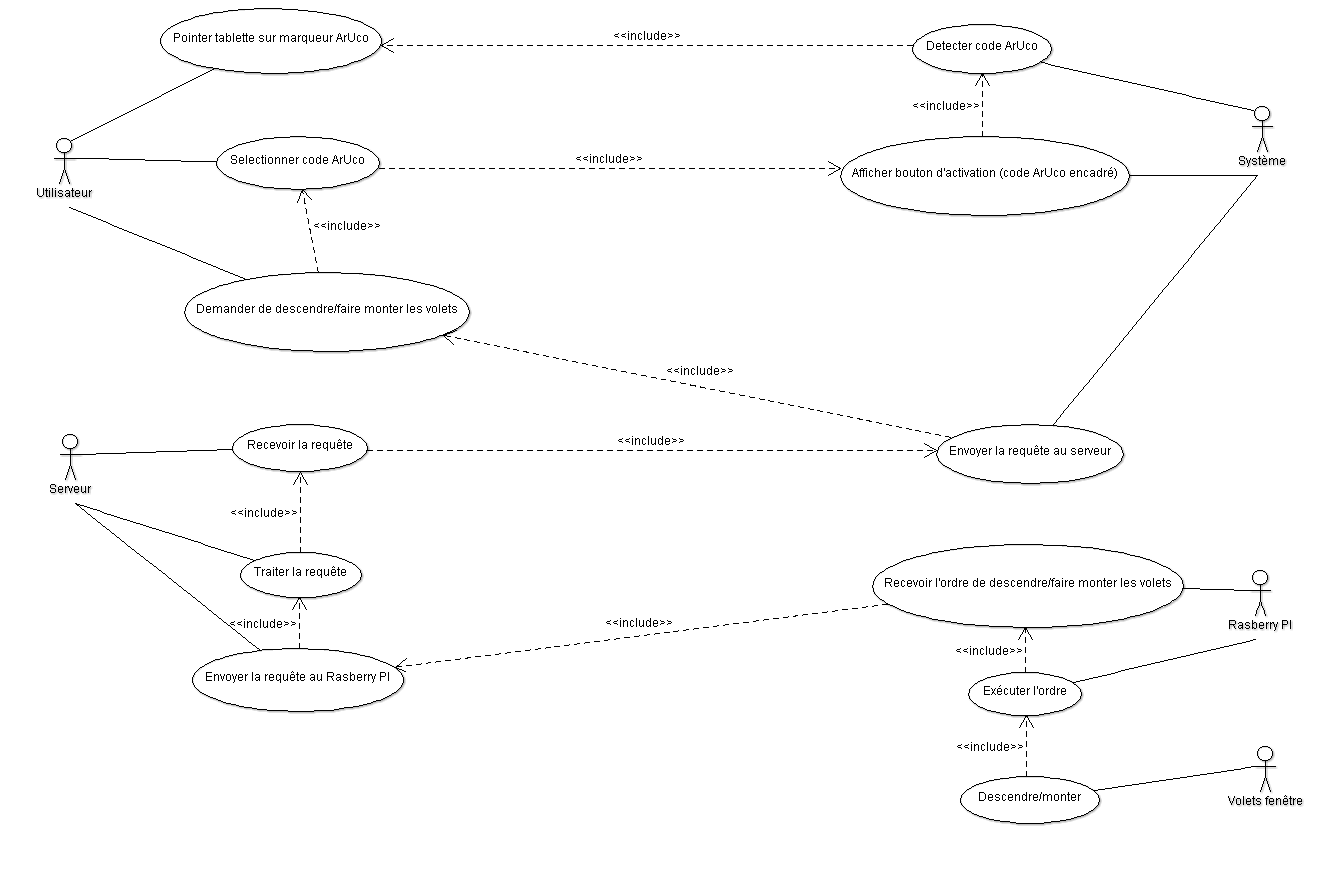
\includegraphics[width = 15cm,height=20cm]{DCU_Fenetre.png}
  \caption{Diagramme de cas d'utilisations d'une fenêtre}
\end{figure}
\newpage
\subsubsection{Cas d'un téléviseur}
\begin{itemize} 
  \item L'utilisateur pointe sa tablette sur un marqueur ArUco.
  \item Le système détecte le code ArUco et y affiche un bouton d'activation. 
  \item L'utilisateur sélectionne le code ArUco en cliquant sur le bouton spécifique.
  \item Le système affiche une interface spécifique au téléviseur.
  \item L'utilisateur demande de changer de chaîne via l'application.
  \item Il peut aussi demander de modifier le son.
  \item Il peut aussi demander d'allumer ou d'éteindre le téléviseur. 
  \item Le système envoie la requête au serveur web.
  \item Le serveur traite la requête et l'envoie au Raspberry PI.
  \item Le Raspberry PI exécute l'ordre selon le choix de l'utilisateur.
\end{itemize}
\newpage
\begin{figure}[h!]
  \centering
  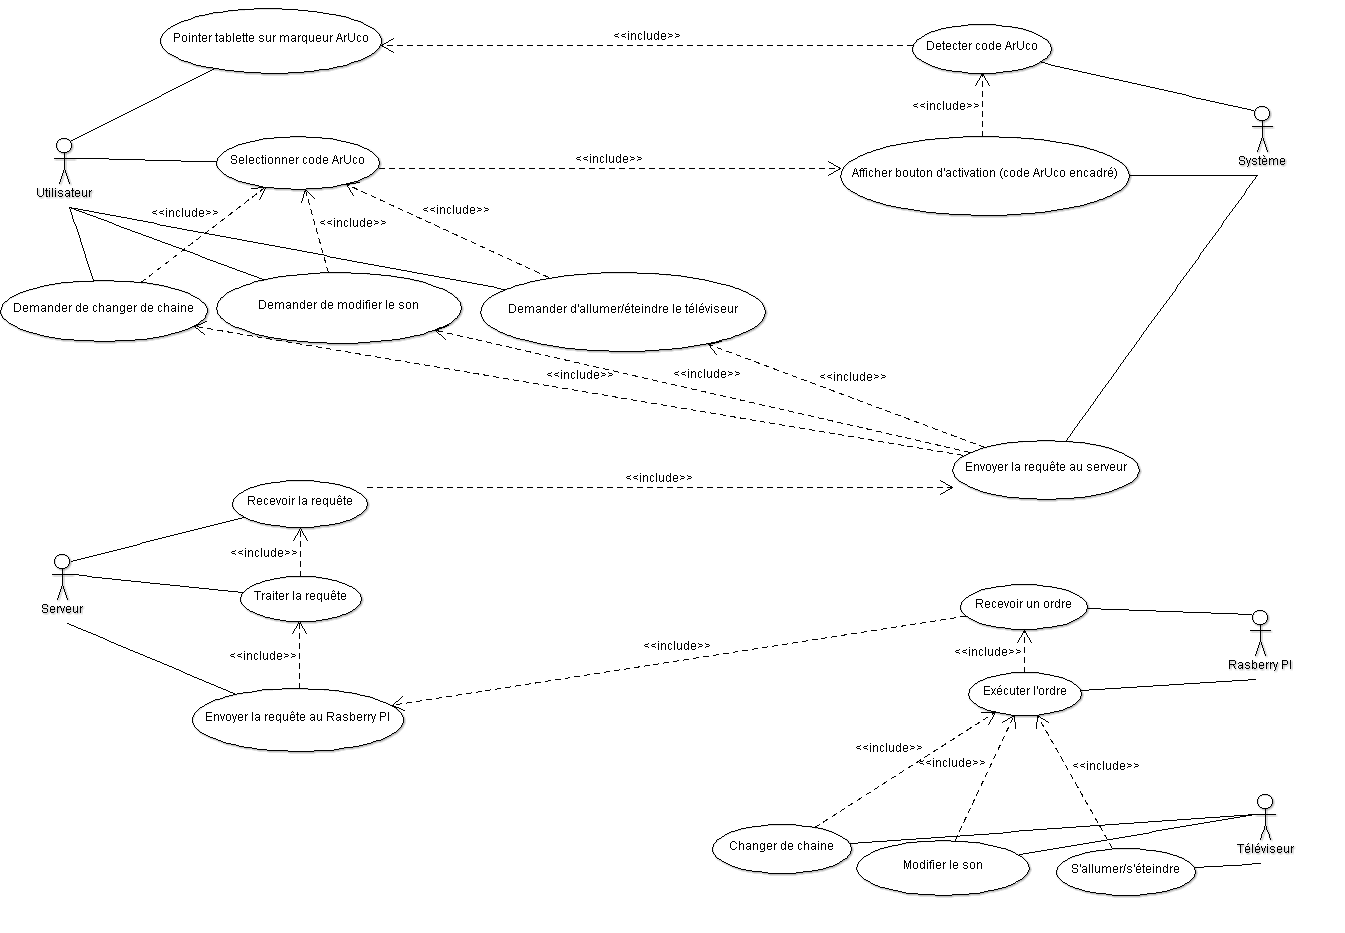
\includegraphics[width = 15cm,height=20cm]{DCU_Televiseur.png}
  \caption{Diagramme de cas d'utilisations d'un téléviseur}
\end{figure}
 \listoffigures
 \newpage
  \bibliography{rapport.bib} %ref au fichier bib
\end{document}
